% !TeX program = lualatex
% IJDAR (Springer Nature) submission build. Figures are shared with ../ (paper/).
\documentclass[sn-mathphys-ay]{sn-jnl}

\usepackage{fontspec}
\setmainfont{Noto Serif}
\newfontfamily\bengalifont{Noto Sans Bengali}[Script=Bengali,Language=Bengali]
\newcommand{\bn}[1]{{\bengalifont #1}}

\usepackage{amsmath}
\usepackage{amssymb}
\usepackage{graphicx}
\graphicspath{{../}}
\usepackage{booktabs}
\usepackage{array}
\usepackage{calc}
\usepackage{textcomp}
\usepackage{listings}
\lstset{basicstyle=\ttfamily\small,breaklines=true,columns=fullflexible,frame=tb,captionpos=t}
\emergencystretch=3em

\begin{document}

\title[Single-Corpus Accuracy Overstates Bengali Compound-Character Recognition]{Single-Corpus Accuracy Overstates Bengali Compound-Character Recognition: A Unified 256-Class Benchmark and Cross-Corpus Evaluation}

\author[1]{\fnm{Uthsob} \sur{Chakraborty}}\email{chakraborty2305341621@diu.edu.bd}
\author[1]{\fnm{Tonmoy} \sur{Biswas}}\email{biswas2305341006@diu.edu.bd}
\author[1]{\fnm{Md. Shihab} \sur{Uddin}}\email{uddin2305341102@diu.edu.bd}
\author[2]{\fnm{Utshob} \sur{Bose}}\email{utshob.bose@g.bracu.ac.bd}
\author*[1]{\fnm{Md. Fahad} \sur{Hossain}}\email{fahadhossain.swe@diu.edu.bd}

\affil[1]{\orgdiv{Department of Software Engineering}, \orgname{Daffodil International University}, \city{Dhaka}, \country{Bangladesh}}
\affil[2]{\orgname{BRAC University}, \city{Dhaka}, \country{Bangladesh}}

\abstract{Bengali compound characters, formed by conjoining two or more consonants, comprise more than 170 mutually confusable glyphs, and progress is held back by fragmented, individually small corpora more than by architecture. Three public corpora (RAS-Compound, Ekush, and MatriVasha) are unified into a 256-class benchmark of 681,309 images, with labels reconciled by Unicode NFC normalisation rather than dataset-local folder indices; the resulting imbalance is an artifact of source size, not character frequency. Four architectures are benchmarked under one protocol: a from-scratch CNN, fine-tuned ResNet18 and ViT-B/16, and ExtendedViT, a hybrid that tokenises images with an ImageNet-pretrained ResNet18 for a four-layer Transformer encoder. ViT-B/16 leads at an equal data budget (0.9662); on the full corpus, ResNet18 and ExtendedViT are indistinguishable (0.9764 vs 0.9760). The most consequential result comes from cross-corpus testing. When a model is trained on one constituent corpus and tested on another, restricted to shared classes, every model falls from 0.96--1.00 same-corpus accuracy to 0.02--0.05, at or barely above chance, and a label-consistency check attributes this to domain shift rather than label disagreement. Single-corpus accuracy therefore reflects familiarity with the corpus, not character recognition. A controlled sweep from 50 to 1,000 images per class, across three seeds, finds no significant accuracy difference between ResNet18 and the hybrid, and the hybrid's raw calibration error, roughly half ResNet18's at small budgets, confers no consistent advantage once both models are temperature-scaled. Warm-starting inflated one result by 1.43 points, and macro-F1 fails to measure long-tail performance when rarity is confounded with source.}

\keywords{Bengali handwritten character recognition, compound characters, cross-corpus generalisation, domain shift, benchmark, Vision Transformer, hybrid CNN--Transformer, model calibration}

\maketitle

\hypertarget{introduction}{%
\section{Introduction}\label{introduction}}

Bengali has about 284 million speakers \citep{ekushnetnote} and is the seventh most spoken language in the world. The script is an abugida with 11 vowels, 39 consonants and 10 numerals, plus an open set of compound characters in which two or more consonants are conjoined. Once diacritics and modifiers are counted, roughly 13,000 grapheme variations are possible \citep{ref30,ref32}. More than 170 of them are conventionally treated as distinct conjunct classes \citep{ref7}.

Handwritten Bengali is hard to recognise for reasons the literature keeps returning to. A cursive head-line binds characters into one visual unit. Two conjuncts can differ by a single stroke or dot. Writing styles vary widely. And because character frequency roughly follows Zipf's law, many compound classes have only a handful of samples \citep{ref33}.

Compound characters concentrate all of these difficulties. Classical
feature-engineering approaches reached only 79--87\% on compound
benchmarks \citep{ref2,ref3,ref4,ref5}, and although deep convolutional networks
lifted this to 90--99\% depending on dataset balance \citep{ref9,ref16,ref23}, the reported ceiling is strongly dependent on how balanced and
how large the evaluation set is. The Vision Transformer \citep{ref22} has
since been shown to outperform VGG-16 and ResNet-50 on Bengali
\emph{basic} characters (98.26\% against 94.54\% and 93.12\%
respectively \citep{ref17}), but its application to compound characters
remains sparse, and Parvez et al.~explicitly identify this as a critical
research gap.

Two considerations complicate a naive transfer of
ViT to this problem. First, ViT lacks the translation
equivariance and locality that convolutions encode
as architectural priors, and consequently underperforms comparably sized ResNets when training data
is merely mid-sized rather than web-scale \citep{ref22}. Bengali compound-character data
is emphatically not web-scale. Second, the available
corpora are fragmented: each is collected under
different conventions, at different resolutions, with
different and only partially overlapping class inventories, so no single one of them supports a large-scale
study.

This paper makes four contributions, and they are
connected: the benchmark is what made the remaining three measurable.

\textbf{Unified benchmark.} RAS-Compound, Ekush, and MatriVasha are combined into one
corpus, which has 256 classes and 681,309 images due to the correspondence of labels on the level of Unicode-normalized graphemes of
Bengali script, instead of dataset-specific folder structure (Section 3.2). To the authors' knowledge, this is the largest unified set of isolated Bengali characters assembled for compound-character classification.
This paper offers not only a compilation of the corpus, but also a characterization of it,
as the imbalance stems from the size of the source, not character frequencies (Section 3.2), but the most significant finding of this work is that models trained on any of the corpora transfer to another \emph{at chance} (Section 4.6). Thus, none of Bengali corpora is capable of training a generalized model, and the merging should be re-interpreted as domain coverage.

\textbf{Four architectures under one protocol.} A from-scratch CNN, a
fine-tuned ImageNet ResNet18, a fine-tuned ViT-B/16, and the hybrid architecture, all
trained and evaluated on a byte-identical split at two data budgets, ViT-B/16 at the equal budget only (Section 4.1).

\textbf{A hybrid architecture, evaluated and not sustained.} ExtendedViT uses an ImageNet pre-trained ResNet18 as a learned tokeniser feeding input into a Transformer encoder (Section 3.4). The thorough sweep on a single corpus, performed using class budgets varying from 50 to 1,000 and different seeds, does not provide \emph{any improvement of accuracy regardless of the budget}, whereas the observed double calibration improvement can be entirely accounted for by temperature scaling and, therefore, is not architectural (Section 4.5).
We thus list it here as a baseline.
The only advantage of this architecture is speed,
with 13 ms CPU inference per image as compared with 45 ms of ViT-B/16 with one point of lower accuracy.

\textbf{Three methodological caveats.} Each of these three warnings comes as a result of falsification efforts against the statements of this study.
\emph{Initialisation:} Both pretrained models inherited previously trained Bengali weights,
which inflated the equal-budget result by 1.43 points and raised first-epoch
validation accuracy from 0.867 to 0.953 (Section 4.9).
\emph{Macro-F1:} In this dataset the rarest classes have the
\emph{highest} F1 scores because class frequencies are confounded with image quality,
so macro-F1 is not a suitable tail metric (Section 4.11).
\emph{Calibration:} Any discrepancies in architecture-specific ECEs can always be fixed after the fact,
and should always be temperature scaled (Section 4.5).

\hypertarget{literature-review}{%
\section{Literature Review}\label{literature-review}}

\hypertarget{introduction-to-bangla-handwritten-character-recognition-and-its-challenges}{%
\subsection{Introduction to Bengali Handwritten Character Recognition
and Its
Challenges}\label{introduction-to-bangla-handwritten-character-recognition-and-its-challenges}}
Of the roughly 284 million Bengali (Bangla) speakers counted in Section 1, about 242 million are native speakers and about 43 million use it as a second language \citep{ekushnetnote}. The script consists of 50 basic characters supplemented with more than 170 conjunct consonants made up of combination of two or more basic characters \citep{ref7}.

Recognition of handwritten characters in the Bengali language is especially difficult due to certain challenges that are repeatedly mentioned in the reviewed literature: (i) cursive nature of the script and head-line connections; (ii) extremely high inter-class similarity when two distinct characters can differ by just one dot \citep{ref32}; (iii) significant variability in handwriting style of each individual writer; (iv) shortage of data on rare compound characters; and (v) unbalanced data distribution because of Zipfian-like frequency distribution of characters in natural Bengali text \citep{ref33}.

These issues make Bengali a classic case of a complex, low-resource script for which OCR/HCR systems still lag behind those developed for Latin scripts \citep{ref21,ref26}.

\hypertarget{traditional-and-classical-methodologies}{%
\subsection{Traditional and Classical
Methodologies}\label{traditional-and-classical-methodologies}}

The earliest work done in Bengali HCR has focused on manually designed
features: gradient and direction features with MQDF classifier
\citep{ref1}; shadow, longest run, and quad-tree features with MLP/SVM,
giving 87.26\% accuracy on a combined set of basic, compound, and modifier
characters \citep{ref2}; CMATERdb 3.1.3.3 dataset itself, which was proposed by
using convex hull and quad-tree features with SVM on 171 compound character
classes with 79.35\% accuracy \citep{ref3}; multi-objective region sampling with
non-dominated sorting harmony search approach, giving 86.65-87.28\%
accuracy \citep{ref4}, later extended to a multi-scale deep quad-tree approach
over several Indic scripts \citep{ref5}; and a two-step MQDF-MLP approach giving
95.8\% accuracy on 50 basic characters \citep{ref6}. In the context of digits,
HOG features along with SVM has provided 98.08\%, 95.68\% and 93.32\% accuracy on CMATERdb, Ekush, and NumtaDB datasets respectively
\citep{ref34}.
All such classical methods are script and feature-engineering based,
scale poorly for the complete set of over 230 characters, and perform at around 79-87\%, which is significantly inferior to deep-learning based approaches;
and their single advantage of low data requirement does not make up for their bad accuracy performance \citep{ref26}.

\hypertarget{cnn-based-deep-learning-approaches}{%
\subsection{CNN-Based Deep Learning
Approaches}\label{cnn-based-deep-learning-approaches}}
CNNs dominated the field of Bengali HCR from about 2015.
Accuracy levels kept rising: 85.36\% by early BHCR-CNN \citep{ref7};
90.33\% by layer-wise DCNN on CMATERdb 3.1.3.3 (171 compound classes)
\citep{ref9}, roughly 10 points higher than previous shallow SVM
benchmarks; 91.23\% by DCNN on BanglaLekha-Isolated \citep{ref10};
96.12\% in 47 epochs after ImageNet-pretrained ResNet-50 and transfer
learning was employed \citep{ref11}; 96.99\% by
InceptionResNetV2/DenseNet121 \citep{ref12}, and a more efficient
MobileNetV1 was used on basic, compound and numeral character classes
\citep{ref13}; 98.03\% by an 11-layer CNN \citep{ref14}; 92.61\% for
Borno, using multiclass CNN training on about one million images
\citep{ref15}; and 99.82\% by squeeze-and-excitation ResNeXt focused
on compound characters \citep{ref16}. Alom et
al.~\citeyearpar{ref8} benchmarked DenseNet, VGG, ResNet, FractalNet,
All-Conv, and Network-in-Network on CMATERdb dataset, where DenseNet
emerged as best; Chakraborty et al.~\citeyearpar{ref58} compared a simple
CNN, deeper DCNN and VGG-16, where DCNN achieved 93.07\%. Among more
recent CNN research we may mention BanglaNet, an ensemble of
Inception/ResNet/DenseNet networks \citep{ref35}; VashaNet, which is a 26-layer CNN achieving 94.43--94.60\% accuracy in two datasets
\citep{ref36}; and CharCrop-GAN, combining contour-based extraction with GAN-based data augmentation along with introducing the 81-class Bangla52 dataset consisting of 24,287 images \citep{ref37}. Despite all progress, CNN-based algorithms have shown their tendency for overfitting to small and imbalanced Bengali datasets, being expensive, and suffering from similar compound characters recognition \citep{ref17,ref23}.

\hypertarget{vision-transformer-and-transformer-based-approaches}{%
\subsection{Vision Transformer and Transformer-Based
Approaches}\label{vision-transformer-and-transformer-based-approaches}}

The foundational Vision Transformer (ViT) \citep{ref22} splits an image
into fixed-size patches (typically 16×16 pixels) treated as tokens for a
standard Transformer encoder. Dosovitskiy et al.\ show that ViT
pretrained on JFT-300M outperforms ResNet baselines at lower
pretraining compute (88.55\% top-1 on ImageNet, 94.55\% on CIFAR-100),
but that this advantage is scale-dependent: on ImageNet-1k alone
ViT-Base trails a comparably sized ResNet; with ImageNet-21k the two
become comparable; only at JFT-300M scale does ViT's inductive-bias-free
design pay off. This finding, that large-scale pretraining compensates
for the convolutional inductive biases ViT lacks, directly motivates
transfer-learning strategies for low-resource scripts such as Bengali.

Parvez et al.~\citeyearpar{ref17} directly compared ViT against VGG-16
and ResNet-50 on CMATERdb 3.1.2 (50 basic characters), with ViT reaching
98.26\% against 94.54\% and 93.12\%, an advantage Parvez et al.\ attribute to ViT's global receptive field; they explicitly flag that ViT ``has not
yet been systematically applied to Bangla handwritten characters'' as a
critical gap. Other Bengali ViT work includes BornoViT, a lightweight
(0.65M-parameter) ViT pretrained on Ekush for resource-constrained
deployment \citep{ref18}; ResViT, which fuses ResNet50v2 and ViT
backbones to reach 97.21\% on BanglaLekha-Isolated \citep{ref19}; and an
eight-layer ViT-only model evaluated on a 15,000-image CMATERdb subset
\citep{ref38}. At the text level, GraDeT-HTR combines a grapheme-based
tokeniser with a decoder-only Transformer for state-of-the-art results
on BN-HTRd and Bongabdo \citep{ref20}, and a CRNN with DenseNet121+GRU
reaches CER 0.091 on BanglaWriting using a 72-basic-class tokeniser that
excludes compound characters \citep{ref39}.

Most closely related to the present work, Hasan, Dhakal, Mehedi, and
Rasel \citep{ref21} propose a TrOCR-style encoder-decoder, an
ImageNet-pretrained ViT encoder with a multilingual text decoder,
fine-tuned on BanglaWriting and a small Nepali dataset (CER 0.07 for
Bengali). This is the closest existing application of an
ImageNet-pretrained ViT to Bengali handwriting, but it operates at the
word level rather than isolating compound-character classification.
Raquib et al.~\citeyearpar{ref25} instead fuse EfficientNetB3, ViT, and a
Conformer branch via cross-attention, reaching 98.84\% on their own
78-class dataset and generalising to 96.49\% on the external CHBCR
benchmark.

Two further architectural extensions bear on the design that follows:
DeiT's data-efficient training (RandAugment, Mixup, CutMix, and
distillation against a CNN teacher) reaches 81.8\% top-1 on ImageNet-1k
without web-scale pretraining \citep{ref41}, relevant given Bengali's
limited labelled data; and the Swin Transformer's shifted-window
attention achieves linear complexity in image size while remaining well
suited to fine structural detail \citep{ref42}. Hybrid designs such as
ResViT \citep{ref19} and the EfficientNetB3--ViT--Conformer model
\citep{ref25} combine local convolutional features with global attention
\emph{in parallel}.

\hypertarget{compound-character-recognition}{%
\subsection{Compound Character
Recognition}\label{compound-character-recognition}}

Studies consistently treat compound characters as a harder problem than basic characters. CompoundDenseNet, a modified DenseNet with enhanced feature reuse, reaches 98.5\%, 98\%, and 96.2\% on BanglaLekha-Isolated, Ekush, and CMATERdb respectively \citep{ref23}, and its authors call for larger and more diverse compound-character datasets. A confidence-guided diffusion augmentation pipeline improves ResNet50, DenseNet121, VGG16, and ViT backbones on the AIBengali dataset, but the best result (VGG16, 89.2\%) is notably lower than balanced-set results elsewhere \citep{ref24}. Shape-decomposition segmentation reduces the effective class count by splitting glyphs into shape components \citep{ref43}. Two other approaches are a two-phase pretrain-then-classify DCNN scheme \citep{ref35} and a HOG-CNN hybrid \citep{ref44}.

The same four challenges recur across these studies. Conjuncts are structurally complex, since each combines two or more basic characters. Inter-class similarity is very high and the glyphs are morphologically diverse. Class imbalance is severe: CMATERdb's compound set is explicitly unbalanced, while BanglaLekha-Isolated has near-uniform classes \citep{ref27}. Finally, data across the 170+ compound classes is limited and fragmented.

\hypertarget{imagenet-pretraining-and-transfer-learning-for-vision-transformers}{%
\subsection{ImageNet Pretraining and Transfer Learning for Vision
Transformers}\label{imagenet-pretraining-and-transfer-learning-for-vision-transformers}}

ImageNet transfer learning is already common practice in Bengali HCR. An ImageNet-pretrained ResNet-50 reached 96.12\% in 47 epochs \citep{ref11}, and transfer learning with InceptionResNetV2 and DenseNet121 reached 96.99\% \citep{ref12}. The TrOCR-style system's ImageNet-pretrained ViT encoder \citep{ref21} applies the same idea to a transformer backbone. Data-efficient training strategies such as DeiT \citep{ref41} could help further with Bengali's data scarcity. One caveat recurs: transfer-learned models can become biased toward source-domain features, which may limit robustness to Bengali-specific script characteristics \citep{ref17}. That caveat is one reason this study tests extended and hybrid ViT designs instead of relying on off-the-shelf fine-tuning alone.

\hypertarget{cross-dataset-evaluation-and-domain-generalisation}{%
\subsection{Cross-Dataset Evaluation and Domain
Generalisation}\label{cross-dataset-evaluation-and-domain-generalisation}}

Most Bengali HCR studies train and evaluate \emph{within} a single corpus, drawing the train/test split from the same collection, so the reported accuracies describe within-corpus competence. Some studies do report results on several benchmarks: BanglaNet \citep{ref35} on CMATERdb, BanglaLekha-Isolated and Ekush; CompoundDenseNet \citep{ref23} on the same three, at 96.2--98.5\%; and Borno \citep{ref15}, trained on roughly one million images drawn from several datasets. In each case the model is trained and tested on each corpus separately. That is multi-benchmark \emph{reporting}. It shows an architecture works on several datasets when trained on each, and says nothing about whether a model trained on one generalises to another.

Genuine held-out-corpus evaluation is rare. The clearest instance in the
reviewed literature is Raquib et al.~\citeyearpar{ref25}, who train on their own
78-class dataset and evaluate on the external CHBCR benchmark, reporting
96.49\% against 98.84\% in-domain, a drop of roughly two points,
which would suggest that cross-dataset transfer is largely intact. A
systematic train-on-one, test-on-another study across
the major Bengali isolated-character corpora was not identified in the reviewed literature, and Section 4.6 of this
paper reports a substantially different picture when one is run.

The wider computer-vision literature has long held that dataset-specific
bias inflates within-dataset performance. Torralba and Efros \citeyearpar{ref45}
showed that a classifier can identify which of several standard datasets
an image came from with high accuracy, a direct demonstration that
datasets carry signatures unrelated to their nominal content, and
that models trained on one dataset degrade markedly when evaluated on
another purporting to cover the same categories. Recht et al.~\citeyearpar{ref46}
found measurable accuracy drops for ImageNet classifiers on a newly
collected test set constructed to follow the original protocol,
indicating that even careful replication of a collection procedure
shifts the distribution. Domain adaptation theory \citep{ref47} formalises
this: generalisation error on a target domain is bounded by source error
plus a divergence term between the domains, so arbitrarily low source
error does not constrain target error when the divergence is large (see
\citep{ref57} for a broader survey of the domain-generalisation
literature).

For handwriting specifically the sources of divergence are concrete and
well understood: capture device and resolution, binarisation and ink
polarity, writing instrument, paper, and, most importantly, the
writer population, since each corpus recruits a distinct set of
contributors with their own regional and generational script
conventions. Section 3.2 documents exactly these differences among the
three corpora merged here: RAS-Compound stores high-resolution binarised
white-on-black glyphs, Ekush is natively 28×28, and MatriVasha is
black-on-white.

This gap is methodological. If within-corpus accuracy is the only metric the field reports, and it substantially overstates performance on newly collected handwriting, then a decade of reported improvements may partly reflect better fitting of corpus-specific signatures. Testing that requires held-out-corpus evaluation as a standard protocol. To the authors' knowledge it has not been applied systematically to Bengali compound characters, and Section 4.6 addresses it.

Two points from the sections above shape the design that follows. First, Dosovitskiy et al.~\citeyearpar{ref22} show that ViT trails a comparably sized ResNet when trained on ImageNet-1k alone, becomes comparable with ImageNet-21k pretraining, and surpasses it only at JFT-300M scale. Large-scale pretraining outweighs inductive bias, so for a low-resource script a pure ViT is the \emph{least} favourable architecture unless a strong prior is supplied externally. Second, the hybrids that exist for Bengali, ResViT \citep{ref19} and the EfficientNetB3--ViT--Conformer of Raquib et al.~\citeyearpar{ref25}, run CNN and transformer branches \emph{in parallel} and fuse their outputs. ExtendedViT composes them \emph{serially}: convolution produces the token sequence that attention then operates over. The original ViT paper's appendix describes this variant, but it has not been evaluated on Bengali script.

\hypertarget{summary-of-benchmark-datasets}{%
\subsection{Summary of Benchmark
Datasets}\label{summary-of-benchmark-datasets}}

Table 1 lists the principal benchmark datasets used in the reviewed literature, with their scale, class composition, and relevance to compound-character recognition.

\begin{table*}[htbp]
\centering
\footnotesize
\caption{Benchmark datasets for Bengali handwritten
character and grapheme recognition.}
\begin{tabular}{>{\raggedright\arraybackslash}p{(\linewidth - 8\tabcolsep) * \real{0.2000}}
  >{\raggedright\arraybackslash}p{(\linewidth - 8\tabcolsep) * \real{0.2000}}
  >{\raggedright\arraybackslash}p{(\linewidth - 8\tabcolsep) * \real{0.2000}}
  >{\raggedright\arraybackslash}p{(\linewidth - 8\tabcolsep) * \real{0.2000}}
  >{\raggedright\arraybackslash}p{(\linewidth - 8\tabcolsep) * \real{0.2000}}}
\toprule
\begin{minipage}[b]{\linewidth}\raggedright
Dataset
\end{minipage} & \begin{minipage}[b]{\linewidth}\raggedright
Reference (year)
\end{minipage} & \begin{minipage}[b]{\linewidth}\raggedright
Size
\end{minipage} & \begin{minipage}[b]{\linewidth}\raggedright
Classes / composition
\end{minipage} & \begin{minipage}[b]{\linewidth}\raggedright
Notes on compound coverage and balance
\end{minipage} \\
\midrule
CMATERdb (3.1.1 / 3.1.2 / 3.1.3.3) & \citet{das2012gaRegion}; \citet{das2009improvedDescriptor}; \citet{ref3} &
3.1.2: 15,000--24,000 images (50 basic); 3.1.3.3: 34,439 train + 8,520
test & 231 total: 50 basic, 10 numerals, 171--172 compound & Standard
benchmark; compound set (3.1.3.3) is unbalanced and un-normalised in
scale/translation \\
Bangla\-Lekha-Isolated & Biswas et al.~\citeyearpar{ref27} & 166,105 images
(\textasciitilde2,000/class) & 84: 50 basic, 10 numerals, 24 compound &
Near-balanced classes; ages 4--28; hosted on Mendeley Data \\
Ekush & Rabby et al.~\citeyearpar{ref29} & 367,018 characters, 3,086 writers
& 122 classes: vowels, consonants, modifiers, 52 compound, digits
(28×28) & Largest isolated-character set; multi-type \\
NumtaDB & Alam et al.~\citeyearpar{ref30} & 85,000+ images & 10 digits only
& Assembled from 6 sources; digits benchmark \\
Bengali.AI Handwritten Graphemes & Alam et al.~\citeyearpar{ref31} & 411k
curated samples (+900 uncommon test graphemes) & 1,295 unique graphemes
(roots, vowel and consonant diacritics); \textasciitilde13,000 possible
& Multi-target labels; tests out-of-dictionary generalisation \\
BangLa52 & CharCrop-GAN \citep{ref37} & 24,287 images & 81 compound classes &
Purpose-built compound set with GAN augmentation \\
Bangla\-Writing & word-level corpus & 21,234 words, 32,784 characters, 260
writers & 5,470 unique words & Word-level; used by CRNN and TrOCR-style
ViT studies \\
CHBCR & external benchmark & --- & vowels, consonants, numerals,
compound & Used for cross-dataset generalisation testing \\
\bottomrule
\end{tabular}
\end{table*}


\hypertarget{summary-of-prior-methods-and-reported-accuracies}{%
\subsection{Summary of Prior Methods and Reported
Accuracies}\label{summary-of-prior-methods-and-reported-accuracies}}

Table 2 consolidates representative methods discussed above alongside
their architectural category, dataset, and reported performance. Because
datasets, class counts, and evaluation protocols differ substantially
across studies, these figures should be interpreted as within-study
results rather than a directly comparable leaderboard (see Section
2.11).

\begin{table*}[htbp]
\centering
\footnotesize
\caption{Representative prior methods and reported
accuracies.}
\begin{tabular}{>{\raggedright\arraybackslash}p{(\linewidth - 8\tabcolsep) * \real{0.1600}}
  >{\raggedright\arraybackslash}p{(\linewidth - 8\tabcolsep) * \real{0.1300}}
  >{\raggedright\arraybackslash}p{(\linewidth - 8\tabcolsep) * \real{0.2600}}
  >{\raggedright\arraybackslash}p{(\linewidth - 8\tabcolsep) * \real{0.1900}}
  >{\raggedright\arraybackslash}p{(\linewidth - 8\tabcolsep) * \real{0.2600}}}
\toprule
\begin{minipage}[b]{\linewidth}\raggedright
Method (year)
\end{minipage} & \begin{minipage}[b]{\linewidth}\raggedright
Category
\end{minipage} & \begin{minipage}[b]{\linewidth}\raggedright
Architecture
\end{minipage} & \begin{minipage}[b]{\linewidth}\raggedright
Dataset(s)
\end{minipage} & \begin{minipage}[b]{\linewidth}\raggedright
Reported result
\end{minipage} \\
\midrule
Pal et al.~\citeyearpar{ref1} & Classical & MQDF + gradient features &
Bengali compound (138 classes) & 85.90\% \\
Das et al.~\citeyearpar{ref2} & Classical & MLP / SVM (shadow, longest-run,
quad-tree) & Basic + compound + modifier & 87.26\% \\
Das et al.~\citeyearpar{ref3} & Classical & Convex-hull + quad-tree + SVM &
CMATERdb 3.1.3.3 (171 compound) & 79.35\% \\
Sarkhel et al.~\citeyearpar{ref4,ref5} & Classical & Region-sampling
+ SVM & CMATERdb / mixed & 87.28\% / 86.65\% \\
Bhattacharya et al.~\citeyearpar{ref6} & Classical & MQDF + MLP (two-stage)
& 50 basic & 95.8\% \\
Rahman et al.~\citeyearpar{ref7} & CNN & BHCR-CNN & 20,000 basic &
85.36\% \\
Roy et al.~\citeyearpar{ref9} & CNN & Layer-wise DCNN & CMATERdb 3.1.3.3
compound & 90.33\% \\
Chatterjee et al.~\citeyearpar{ref11} & CNN + transfer & ResNet-50
(ImageNet) & Bangla\-Lekha-Isolated & 96.12\% \\
Ghosh et al.~\citeyearpar{ref12} & CNN + transfer & Inception\-Res\-Net\-V\-2 /
Dense\-Net\-121 & CMATERdb & 96.99\% \\
Hasan et al.~\citeyearpar{ref14} & CNN & 11-layer CNN & CMATERdb 3.1.2 &
98.03\% \\
SE-ResNeXt \citep{ref16} & CNN & ResNeXt + SE blocks & Compound set & 99.82\%
(avg) \\
VashaNet \citep{ref36} & CNN & 26-layer CNN & CMATERdb / primary &
94.43\% / 94.60\% \\
Compound\-Dense\-Net \citep{ref23} & CNN (compound) & Modified DenseNet &
Bangla\-Lekha / Ekush / CMATERdb & 98.5\% / 98\% / 96.2\% \\
Diffusion augmentation \citep{ref24} & CNN + ViT (compound) &
Diffusion aug. + SE-ResNet/VGG/ViT & AIBengali compound & 89.2\% (VGG16
best) \\
Parvez et al.~\citeyearpar{ref17} & ViT & ViT vs VGG-16 vs ResNet-50 &
CMATERdb 3.1.2 (basic) & ViT 98.26\% / VGG 94.54\% / ResNet 93.12\% \\
BornoViT \citep{ref18} & Lightweight ViT & 0.65M-param ViT & Ekush /
Bornomala (basic + digits) & Efficiency-focused \\
ResViT \citep{ref19} & Hybrid CNN--ViT & Res\-Net\-50v\-2 + ViT &
Bangla\-Lekha-Isolated & 97.21\% \\
Raquib et al.~\citeyearpar{ref25} & Hybrid (compound) & Efficient\-Net\-B\-3 + ViT
+ Conformer + cross-attention & Own (78-class) / CHBCR & 98.84\% /
96.49\% \\
Safir et al.~\citeyearpar{ref39} & CRNN (word) & Dense\-Net\-121 + GRU + CTC &
Bangla\-Writing & CER 0.091 / WER 0.273 \\
Hasan et al.~\citeyearpar{ref21} & ViT encoder--decoder & ViT (ImageNet) +
xlm-roberta & Bangla\-Writing (Bengali) & Test CER 0.07 / WER 0.12 \\
GraDeT-HTR \citep{ref20} & Decoder-only Transformer & Grapheme
tokeniser + patch-embed decoder & BN-HTRd / Bongabdo & State of the art
(CER/WER) \\
\bottomrule
\end{tabular}
\end{table*}


\hypertarget{research-gaps}{%
\subsection{Research Gaps}\label{research-gaps}}

Synthesising the studies reviewed above, seven overarching gaps emerge
that motivate this study.

First, ViT remains under-applied to compound characters. It excels on
basic characters, reaching 98.26\% accuracy \citep{ref17}, but has rarely
been applied systematically to Bengali, and almost never to isolated
compound characters specifically; Parvez et al.~\citeyearpar{ref17} explicitly
describe this as a critical research gap.

Second, existing transformer work exhibits a basic-character bias.
BornoViT \citep{ref18}, ResViT \citep{ref19}, and the eight-layer ViT model
\citep{ref38} target basic characters or digits, while GraDeT-HTR \citep{ref20},
the CRNN of Safir et al.~\citeyearpar{ref39}, and the TrOCR-style ViT of Hasan et
al.~\citeyearpar{ref21} operate at the word or line level, leaving isolated
compound-character classification comparatively under-explored.

Third, class imbalance and data scarcity for compound characters are
addressed through ad hoc augmentation (GAN-based \citep{ref37} or
diffusion-based \citep{ref24}) rather than through principled transfer
learning, leaving open whether principled transfer learning offers a stronger prior for the long tail of rare conjunct classes.

Fourth, transfer-learning studies specifically for Bengali compound
characters are scarce. ImageNet transfer is well established for CNNs
\citep{ref11,ref12} and for word-level ViT encoders \citep{ref21}, but not for
compound-character ViT classification, and existing transfer-learned
models have been noted to risk bias toward source-domain features
\citep{ref17}, which motivated testing an extended rather than vanilla ViT design here.

Fifth, the field values efficiency alongside accuracy for low-resource
deployment, as demonstrated by BornoViT \citep{ref18} and GraDeT-HTR
\citep{ref20}; any architecture proposed for compound characters should therefore be evaluated on parameter and computational cost as well as accuracy.

Sixth, no existing extended or hybrid ViT architecture has been
specifically tailored to compound-character structural complexity with
ImageNet initialisation, despite the availability of relevant building
blocks such as hybrid CNN--ViT designs \citep{ref19,ref25} and
multi-scale hierarchical transformers \citep{ref42}.

Seventh, and closest to this paper's own contribution: \emph{no
systematic cross-corpus evaluation exists for Bengali handwritten
characters.} Multi-benchmark reporting is common (Section 2.7), but
train-on-one/test-on-another transfer is essentially unmeasured, leaving
open whether reported accuracies reflect character recognition or corpus
familiarity. Section 4.6 addresses this gap directly.

\hypertarget{summary}{%
\subsection{Summary}\label{summary}}

The reviewed literature traces a clear trajectory in Bengali handwritten
character recognition: from handcrafted-feature classifiers (MQDF and
quad-tree or longest-run features combined with SVM or MLP classifiers,
achieving roughly 79--87\% on compound characters \citep{ref1,ref2,ref3,ref4,ref5,ref6}),
through deep CNNs and ensembles (DenseNet, ResNet, Inception,
MobileNet, and SE-ResNeXt architectures, reaching 90--99.8\% depending
on dataset balance \citep{ref7,ref8,ref9,ref10,ref11,ref12,ref13,ref14,ref15,ref16,ref23}), to an emerging Vision
Transformer and hybrid-attention era in which ViT now outperforms
leading CNNs on standard basic-character benchmarks (98.26\% versus
93--95\%) \citep{ref17}, and in which lightweight, grapheme-aware, and
TrOCR-style transformer systems demonstrate the paradigm's breadth
\citep{ref18,ref19,ref20,ref21,ref25}.

Compound characters, however, remain the field's frontier: they are
structurally complex, mutually confusable, imbalanced, and comparatively
data-scarce, and no prior study combines the three elements central to
the present work: ImageNet pretraining, an extended or hybrid ViT
architecture, and an explicit focus on compound characters. The
theoretical grounding for ViT transfer learning, whereby large-scale
pretraining compensates for the inductive biases ViT lacks \citep{ref22},
together with the demonstrated success of ImageNet transfer in Bengali
CNNs \citep{ref11,ref12} and word-level ViT-based OCR \citep{ref21}, and the
data-efficiency techniques offered by DeiT \citep{ref41} and the multi-scale
attention of Swin Transformer \citep{ref42}, collectively motivated the direction tested in this study. Section 4 reports that, on this benchmark, the hybrid does not deliver an accuracy advantage over its own convolutional trunk.

It is worth noting that reported accuracies across the studies discussed
are not directly comparable, owing to differences in datasets (CMATERdb,
BanglaLekha-Isolated, Ekush), class counts (ranging from 50 to 231
classes), train/test splits, image resolutions, and whether numerals and
modifiers are included; the figures in Table 2 should therefore be
read as within-study results rather than a ranked comparison. Several
sources reviewed are non-peer-reviewed preprints, including BornoViT
\citep{ref18}, the multi-head attention model \citep{ref25}, the confidence-guided
diffusion paper \citep{ref24}, and the Bengali/Nepali TrOCR work \citep{ref21},
whose reported figures await peer validation. As established in Section
2.7, none of this prior work measures transfer \emph{across} corpora,
which is where the present paper departs from it.


\hypertarget{methodology}{%
\section{Methodology}\label{methodology}}

\hypertarget{overall-workflow}{%
\subsection{Overall Workflow}\label{overall-workflow}}

Figure 1 shows the end-to-end pipeline: three source corpora \ensuremath{\rightarrow}
grapheme-level label reconciliation \ensuremath{\rightarrow} unified 256-class manifest \ensuremath{\rightarrow}
stratified split \ensuremath{\rightarrow} polarity normalisation and augmentation \ensuremath{\rightarrow} four
architectures trained under an identical protocol \ensuremath{\rightarrow} evaluation on one
shared test set.

\begin{figure}
\centering
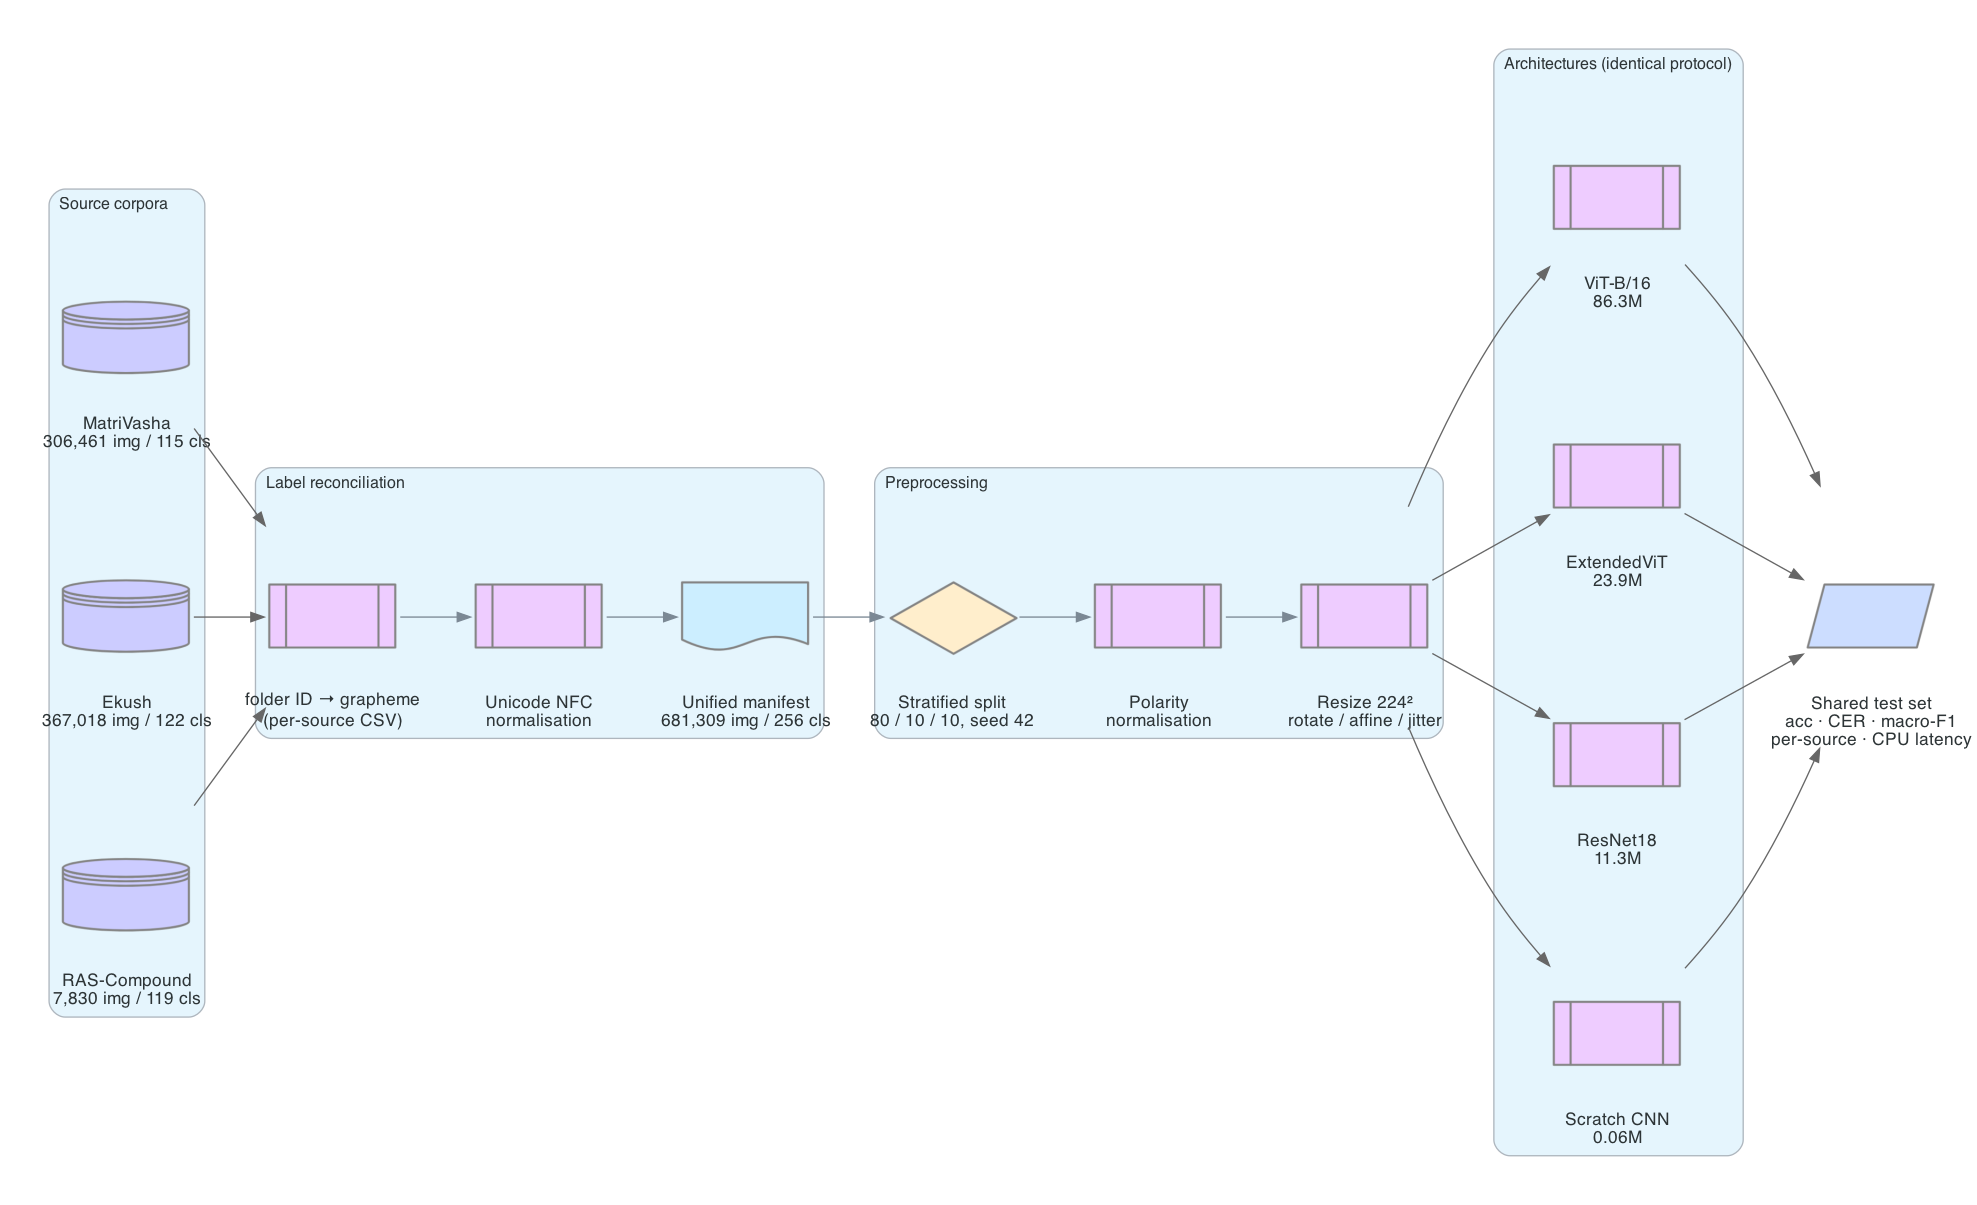
\includegraphics[width=0.85\linewidth]{fig1_workflow.png}
\caption{Overall workflow: three corpora, grapheme-level label
reconciliation, one shared split, four architectures, one test set.}
\end{figure}

The pipeline is deliberately organised so that every architecture
consumes byte-identical data. Dataset scanning, label reconciliation,
splitting, and image transformation are implemented once and shared; the
architecture is the only variable that changes between runs. This
matters because the comparisons in Sections 4.2--4.4 turn on differences of one
to two accuracy points, which are easily manufactured by an inconsistent
split.

\hypertarget{dataset}{%
\subsection{Dataset}\label{dataset}}

Three corpora are combined. RAS-Compound \citep{ref50} is a small,
purpose-built compound-character set distributed as a Kaggle dataset.
Ekush \citep{ref29} is among the largest isolated Bengali character
collections, gathered from 3,086 writers. MatriVasha \citep{ref49}
is a compound-character corpus collected with per-writer gender
metadata, which is not used as a label here but which contributes writer
diversity.

\begin{table*}[htbp]
\centering
\footnotesize
\caption{Composition of the unified corpus.}
\begin{tabular}{>{\raggedright\arraybackslash}p{(\linewidth - 8\tabcolsep) * \real{0.1579}}
  >{\raggedleft\arraybackslash}p{(\linewidth - 8\tabcolsep) * \real{0.2105}}
  >{\raggedleft\arraybackslash}p{(\linewidth - 8\tabcolsep) * \real{0.2105}}
  >{\raggedleft\arraybackslash}p{(\linewidth - 8\tabcolsep) * \real{0.2105}}
  >{\raggedleft\arraybackslash}p{(\linewidth - 8\tabcolsep) * \real{0.2105}}}
\toprule
\begin{minipage}[b]{\linewidth}\raggedright
Source
\end{minipage} & \begin{minipage}[b]{\linewidth}\raggedleft
Images
\end{minipage} & \begin{minipage}[b]{\linewidth}\raggedleft
Classes
\end{minipage} & \begin{minipage}[b]{\linewidth}\raggedleft
Classes unique to this source
\end{minipage} & \begin{minipage}[b]{\linewidth}\raggedleft
Mean images/class
\end{minipage} \\
\midrule
RAS-Compound & 7,830 & 119 & 27 & 66 \\
Ekush & 367,018 & 122 & 80 & 3,008 \\
Matri\-Vasha & 306,461 & 115 & 52 & 2,665 \\
\textbf{Unified} & \textbf{681,309} & \textbf{256} & --- &
\textbf{2,661} \\
\bottomrule
\end{tabular}
\end{table*}


Table 3 gives the composition of each source. Class inventories overlap only partially: 37 classes are shared between
RAS-Compound and Ekush, 58 between RAS-Compound and MatriVasha, 8
between Ekush and MatriVasha, and just 3 appear in all three. 159 of the
256 classes are contributed by exactly one source. The merge is
therefore not a redundant enlargement of an existing set: it
materially extends class coverage, which is the stated need in the
compound-character literature \citep{ref23}.

\textbf{Label reconciliation.} Each source indexes its classes by a
local folder number whose meaning is defined only by that project's own
mapping file. Merging on folder index would conflate unrelated
characters. Instead, every folder is resolved to its Bengali grapheme via the source's mapping (\texttt{ras\_class\_mapping.csv}, Ekush's \texttt{metaData\_img.csv}, \texttt{matrivasha\_mapping.csv}), Unicode NFC normalisation is applied, and the union of the resulting grapheme set is taken as the label space. NFC matters because the same conjunct may be
encoded with different code-point sequences across projects; without
normalisation, visually and semantically identical characters would
occupy separate classes.

Figure 2 shows (a) the sorted per-class frequency curve on a
log axis and (b) the relative contribution of each source.
Figure 3 shows the same three characters as collected by each
corpus, and makes the heterogeneity concrete: RAS-Compound stores
high-resolution white-on-black binarised glyphs, Ekush is natively 28×28
and visibly pixelated when upsampled, and MatriVasha is
\emph{black-on-white}, the opposite ink polarity. Any merge of
these three must reconcile that variation before a single model can
consume them, which is the subject of the next section.

\begin{figure}
\centering
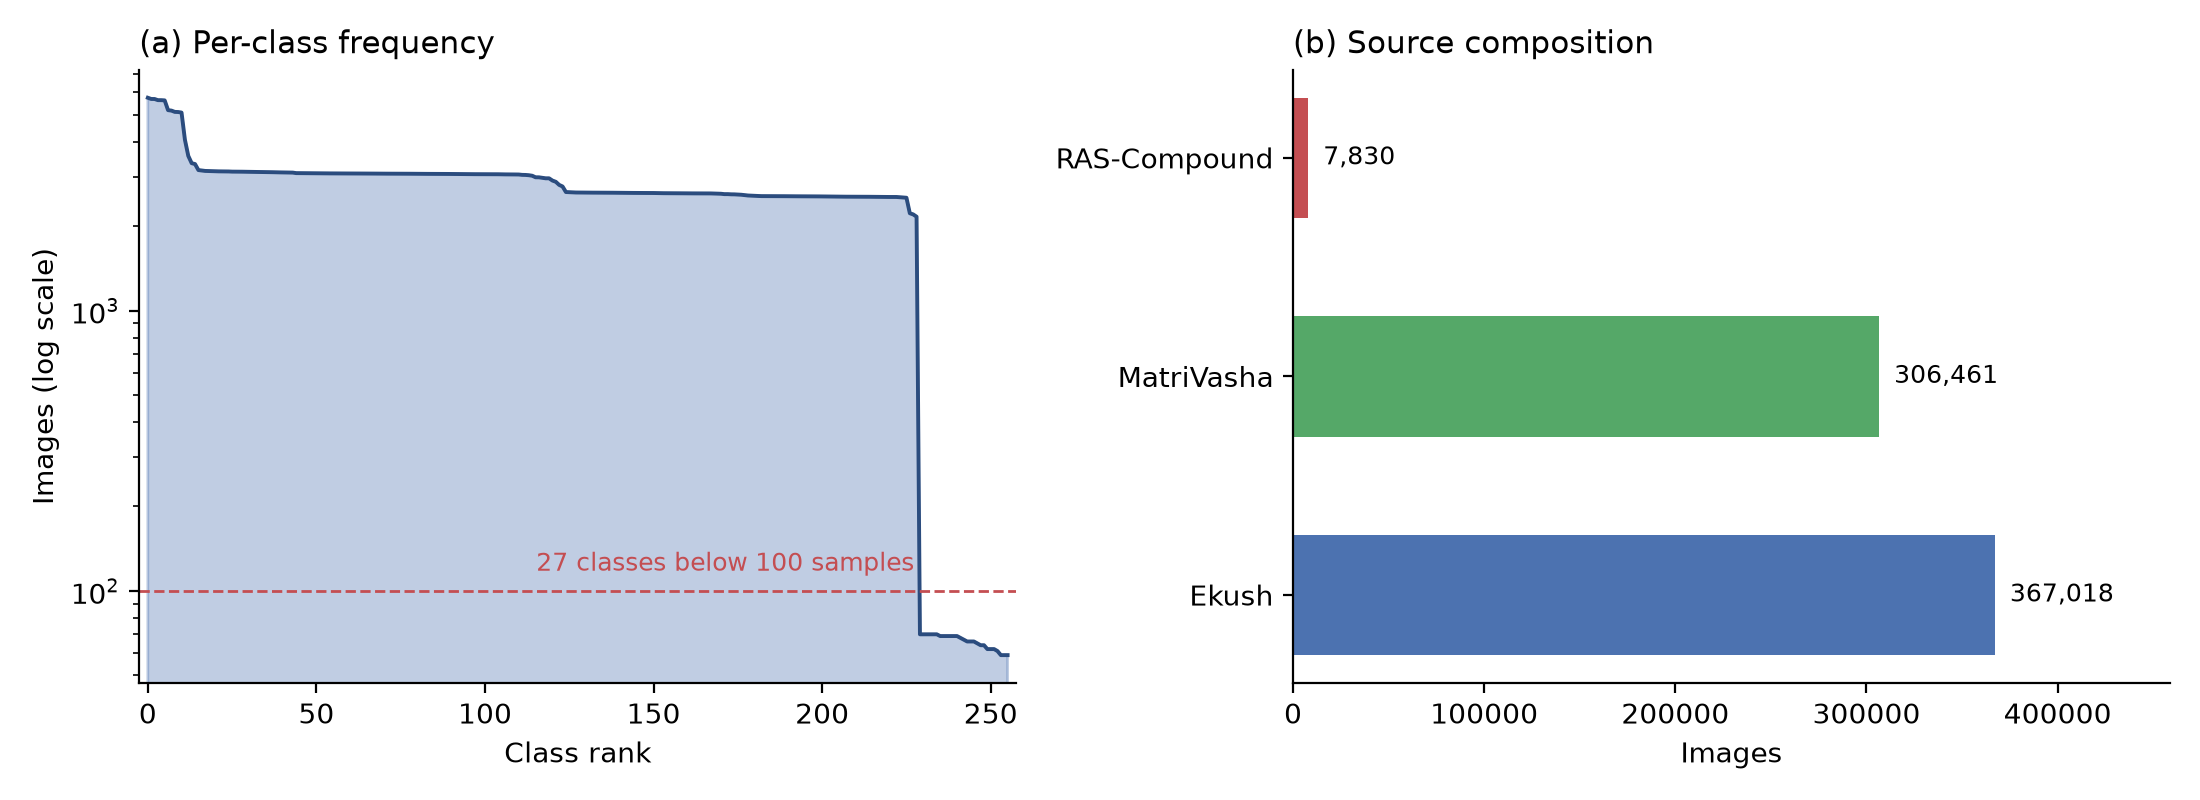
\includegraphics[width=0.85\linewidth]{fig2_dataset.png}
\caption{Dataset composition. (a) Per-class frequency, log
scale. (b) Images contributed by each corpus.}
\end{figure}

\begin{figure}
\centering
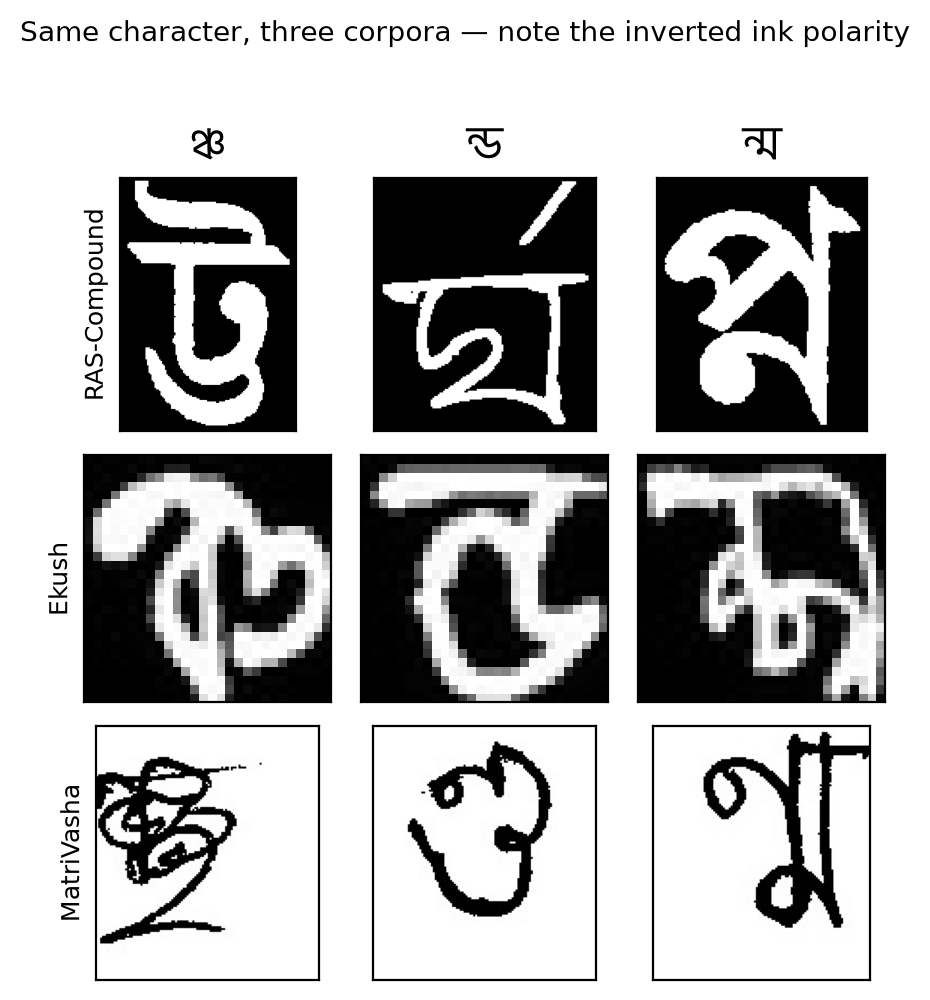
\includegraphics[width=0.85\linewidth]{fig4_samples.png}
\caption{The same three characters as collected by each
corpus. Note the resolution difference and MatriVasha's inverted ink
polarity.}
\end{figure}

\textbf{Class imbalance.} Class frequencies range from 59 to 5,740
images with a median of 2,636. The distribution is not Zipfian, as might
be expected from natural Bengali text frequency \citep{ref33}, but sharply
\emph{bimodal}: 229 classes form a broad, comparatively flat body
between roughly 2,000 and 5,700 samples, and the remaining 27 fall off a
cliff to fewer than 100 (Figure 2a). Those 27 are exactly the classes
contributed uniquely by RAS-Compound, whose 7,830 images spread across
119 classes average only 66 per class.

\textbf{Source of the imbalance.} The imbalance is an artifact of source size, not of character frequency. Each corpus is internally near-balanced: within Ekush,
per-class counts run from 514 to 4,067 with an interquartile range of
just 3,056--3,079; within MatriVasha, 2,548--2,563; within RAS-Compound,
a uniform 34--70. The bimodality in Figure 2(a) therefore arises
entirely from RAS-Compound being a small collection (\ensuremath{\approx}66 images per
class) whose 27 unique classes no other corpus supplies, not from
those conjuncts being intrinsically rarer in written Bengali.

This distinction matters for interpreting any per-class result. Because
class rarity and source identity are perfectly confounded in this corpus
(every low-frequency class is a RAS-Compound class, and RAS-Compound
has a distinctive image convention: high-resolution, cleanly binarised),
a model that performs better on rare classes cannot be shown to
handle \emph{rarity} better rather than simply handling \emph{that
corpus's image style} better. This paper therefore does not claim rare-class
advantage for any architecture, and reports macro-averaged F1
alongside accuracy as a descriptive statistic rather than as evidence
about the long tail. Establishing genuine data-efficiency behaviour
requires controlled subsampling within a single source (Section 4.4).

\hypertarget{preprocessing-and-data-splitting}{%
\subsection{Preprocessing and Data
Splitting}\label{preprocessing-and-data-splitting}}

\textbf{Polarity normalisation.} As Figure 3 shows, the three sources do
not agree on ink polarity: RAS-Compound and Ekush store light ink on a
dark ground, MatriVasha the inverse. Left unaddressed, the same
character would present to the network as two different visual patterns
depending on its source, and the model would be forced to learn each
convention separately. Polarity is normalised by comparing the mean intensity of the image border against the global mean and inverting when the border is brighter, which yields bright ink on a dark ground regardless of
source convention. This is applied before all other transformations.
Figure 4 traces one glyph per source through normalisation and
three augmentation draws; the MatriVasha row shows the inversion taking
effect.

\begin{figure}
\centering
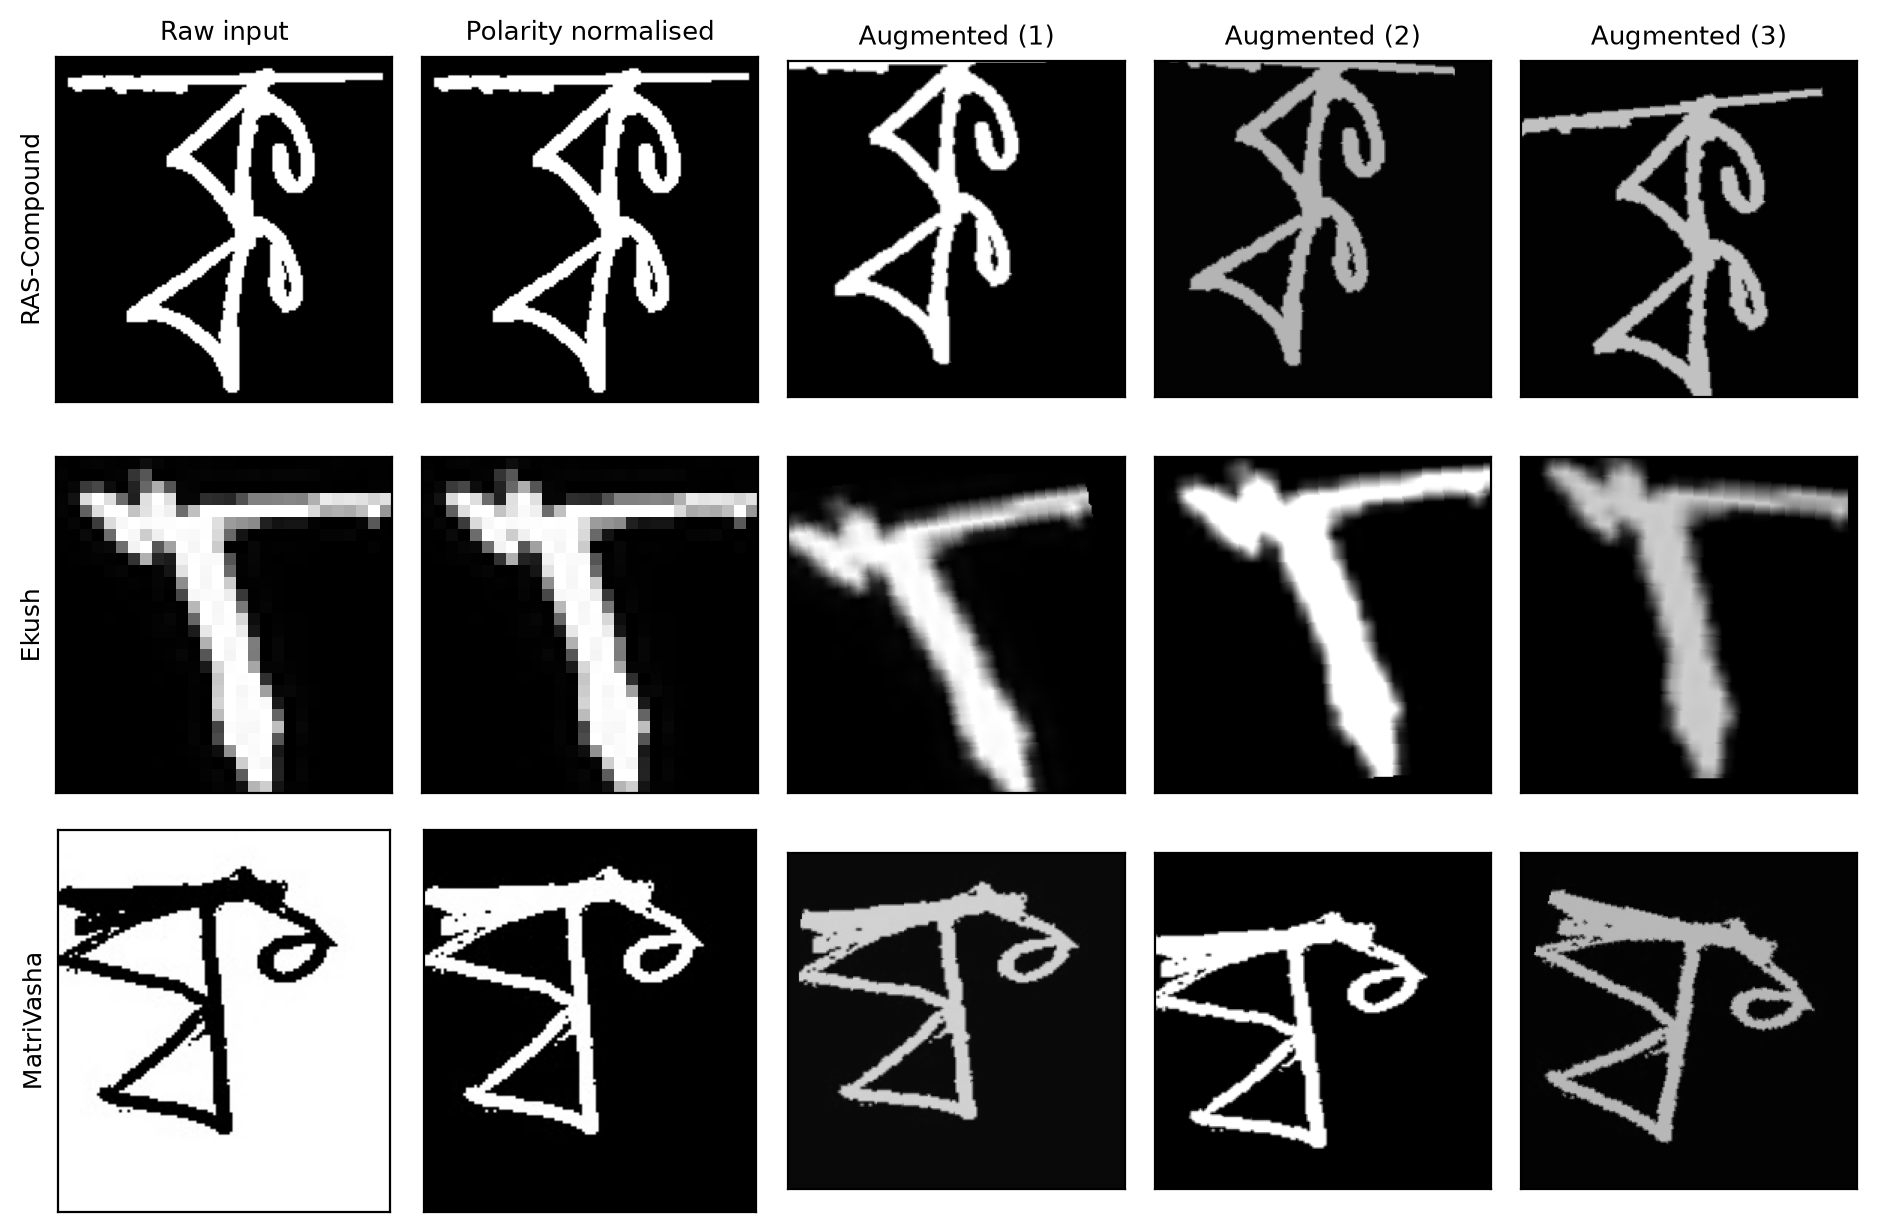
\includegraphics[width=0.85\linewidth]{fig5_preprocessing.png}
\caption{One glyph per corpus through polarity normalisation
and three augmentation draws.}
\end{figure}

\textbf{Transformations.} Images are converted to three-channel
grayscale (the pretrained backbones expect three channels) and resized
to 224×224. Training additionally applies random rotation of ±15°,
random affine translation of up to 10\% with 5° shear, and colour jitter
of 0.3 in brightness and contrast. Horizontal flipping is deliberately
excluded: Bengali characters are direction-sensitive and a mirrored
glyph is not a valid sample of its own class. All images are normalised
to zero mean and unit variance per channel using μ = σ = 0.5.

\textbf{Splitting.} The data are split 80/10/10, stratified per class with a fixed seed, so that rare classes are represented in all
three partitions rather than concentrated in whichever partition chance
assigns them. Classes with fewer than three samples contribute entirely
to training. The full corpus yields 545,289 training, 68,010 validation,
and 68,010 test images. The split is computed once from the manifest and
reused by every architecture; the test partition is never used for model
selection, which is performed on validation accuracy alone.

\hypertarget{proposed-method-extendedvit}{%
\subsection{Hybrid Architecture: ExtendedViT}\label{proposed-method-extendedvit}}

ExtendedViT composes a convolutional backbone and a Transformer encoder
serially, using the former as a learned tokeniser for the latter.

\textbf{Convolutional tokeniser.} An input image
\(x \in \mathbb{R}^{3 \times 224 \times 224}\) is passed through the
convolutional stages of an ImageNet-pretrained ResNet18, up to and
including \texttt{layer4} and excluding the global pooling and
classification head (Eq.~1):

\begin{equation}
F = f_{\text{ResNet18}}(x) \in \mathbb{R}^{512 \times 7 \times 7}
\end{equation}

\textbf{Tokenisation.} The spatial map is flattened along its spatial
axes into a sequence of \(N = 49\) tokens of dimension \(D = 512\),
where each token corresponds to a 32×32-pixel cell of the input (its receptive field is larger)
(Eq.~2):

\begin{equation}
F' = \text{flatten}(F) \in \mathbb{R}^{49 \times 512}
\end{equation}

A learnable classification token
\(x_{\text{cls}} \in \mathbb{R}^{1 \times D}\) is prepended and a
learnable positional embedding
\(E_{\text{pos}} \in \mathbb{R}^{(N+1) \times D}\) is added, following
the Vision Transformer's construction \citep{ref22}:

\begin{equation}
z_0 = [\,x_{\text{cls}}\,;\,F'_1\,;\,F'_2\,;\,\dots\,;\,F'_{49}\,] + E_{\text{pos}}
\end{equation}

Both are initialised from a truncated normal distribution with standard
deviation 0.02, giving the token sequence of Eq.~3.

\textbf{Transformer encoder.} The 50-token sequence passes through
\(L = 4\) post-norm encoder layers, each comprising multi-head
self-attention with \(h = 8\) heads and a position-wise feed-forward
network of inner dimension 2048, with residual connections and layer
normalisation (Eqs.~4--5):

\begin{equation}
z'_\ell = \text{LN}\big(z_{\ell-1} + \text{MSA}(z_{\ell-1})\big)
\end{equation}
\begin{equation}
z_\ell = \text{LN}\big(z'_\ell + \text{FFN}(z'_\ell)\big), \qquad \ell = 1 \dots L
\end{equation}

where multi-head self-attention (Eqs.~6--7) follows the standard
formulation \citep{ref51} over \(h\) heads of dimension
\(d_k = D/h = 64\):

\begin{equation}
\text{MSA}(z) = [\text{head}_1 ; \dots ; \text{head}_h] W^O
\end{equation}

\begin{equation}
\text{head}_i = \text{softmax}\left(\frac{Q_i K_i^{\top}}{\sqrt{d_k}}\right) V_i
\end{equation}

with \(Q_i = zW_i^Q\), \(K_i = zW_i^K\), \(V_i = zW_i^V\). Dropout of
0.1 is applied within each layer.

\textbf{Classification.} The final classification token is
layer-normalised and projected to the label space (Eq.~8):

\begin{equation}
\hat{y} = \text{softmax}\big(W_{\text{head}}\,\text{LN}(z_L^{0}) + b\big), \qquad
W_{\text{head}} \in \mathbb{R}^{256 \times 512}
\end{equation}

\textbf{Design rationale.} Standard ViT tokenises by linear projection
of raw 16×16 pixel patches, which supplies the encoder with no spatial
prior whatsoever and is exactly why ViT needs web-scale pretraining to
compete \citep{ref22}. Substituting a pretrained convolutional stack for that
projection means each token already encodes a locally
translation-equivariant, hierarchically composed feature: ImageNet's
inductive bias arrives with the weights. Attention then operates over 50
tokens rather than the 197 of ViT-B/16, an approximately 15× reduction
in attention cost, which reduces CPU latency relative to ViT-B/16 (Sections 3.6 and 4.7). For compound characters specifically, the motivation is
that a conjunct is defined by the \emph{relationship} between its
constituent consonant forms and their placement relative to the
head-line; convolution captures the constituents, and self-attention
over the full glyph captures the relationship.

Figure 5 shows the data flow with tensor shapes annotated at
each stage, and Table 4 lists the shapes and parameter counts layer by layer.

\begin{figure}
\centering
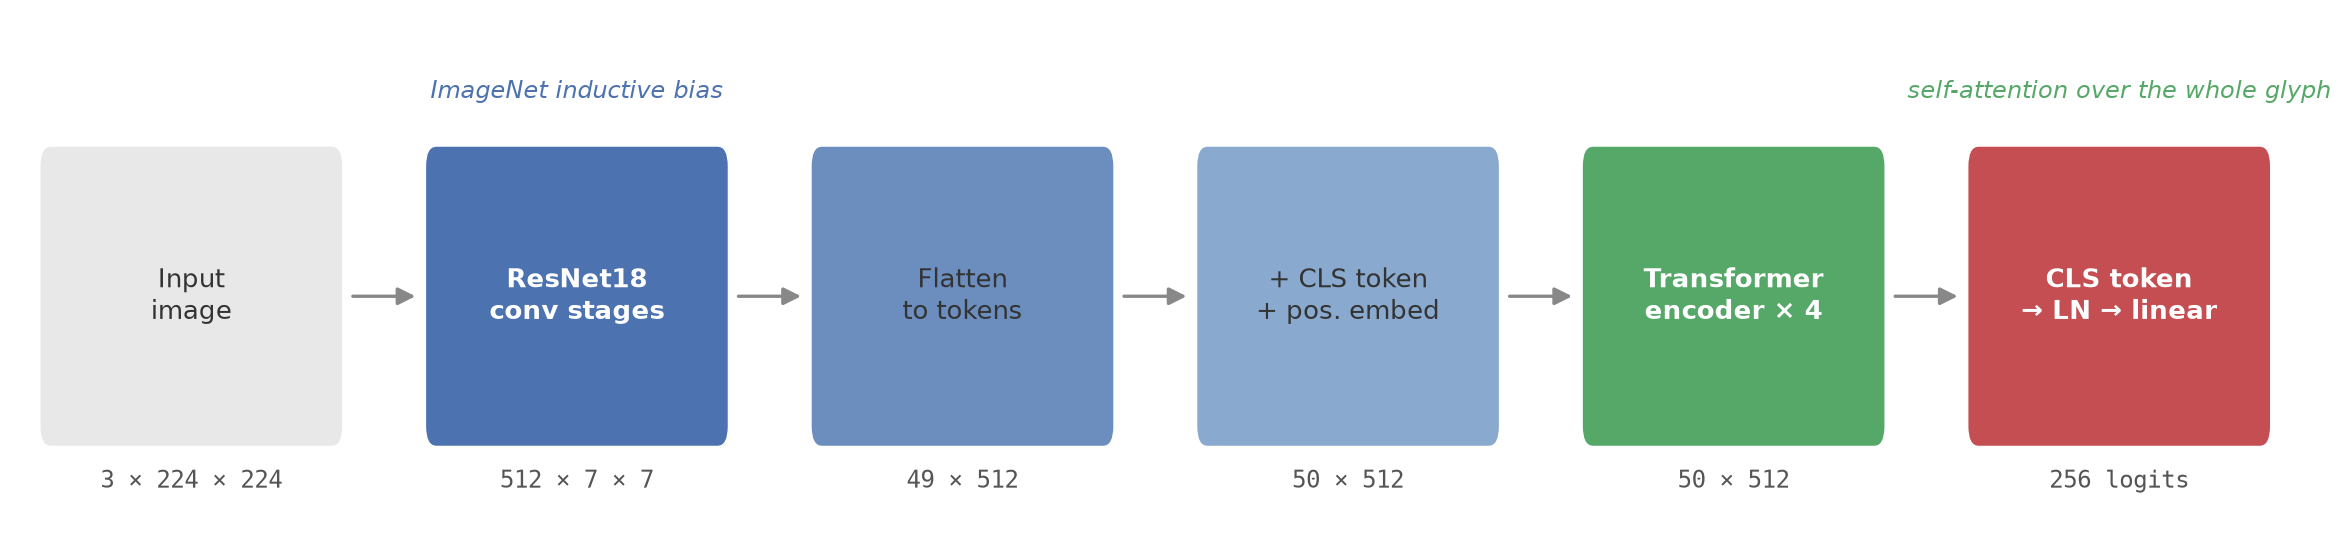
\includegraphics[width=0.85\linewidth]{fig3_architecture.png}
\caption{ExtendedViT: a ResNet18 tokeniser feeding a
four-layer Transformer encoder, with tensor shapes at each stage.}
\end{figure}

\begin{table*}[htbp]
\centering
\footnotesize
\caption{Extended\-Vi\-T layer summary.}
\begin{tabular}{llr}
\toprule
Stage & Output shape & Params \\
\midrule
Input & 3 × 224 × 224 & --- \\
ResNet18 conv1 + bn1 + maxpool & 64 × 56 × 56 & 9,536 \\
ResNet18 layer1--layer4 & 512 × 7 × 7 & 11,166,976 \\
Flatten \ensuremath{\rightarrow} tokens & 49 × 512 & --- \\
CLS token + positional embedding & 50 × 512 & 26,112 \\
Transformer encoder × 4 & 50 × 512 & 12,609,536 \\
LayerNorm + linear head & 256 & 132,352 \\
\textbf{Total} & & \textbf{23,944,512} \\
\bottomrule
\end{tabular}
\end{table*}


\hypertarget{baseline-architectures}{%
\subsection{Baseline Architectures}\label{baseline-architectures}}

Three baselines span the categories identified in the review.

\textbf{Scratch CNN.} A compact separable-convolution network, one
standard 3×3 convolution followed by three depthwise-separable blocks
with max-pooling, global average pooling, and a 128-unit hidden layer,
totalling 62,208 parameters, trained from random initialisation. It
quantifies what is achievable without any transfer learning.

\textbf{ResNet18 (ImageNet).} The same backbone ExtendedViT uses, with a
linear classifier replacing the 1000-way head, fine-tuned end to end. It
is the control that isolates the contribution of the transformer
encoder: any difference between it and ExtendedViT is attributable to
the attention stack, since the convolutional trunk is identical.

\textbf{ViT-B/16 (ImageNet).} A standard Vision Transformer with 16×16
patch embedding and 12 encoder layers (86.3M parameters), fine-tuned
with a custom head. It represents the pure-transformer approach that
Parvez et al.~\citeyearpar{ref17} found superior on basic characters.

\hypertarget{training-configuration-and-inference}{%
\subsection{Training Configuration and
Inference}\label{training-configuration-and-inference}}

\textbf{Optimisation.} All models use AdamW \citep{ref53} with weight
decay 10⁻⁴, cross-entropy loss with label smoothing 0.1
\citep{ref55,ref56}, and a cosine-annealing schedule \citep{ref54}
decaying to 10⁻⁶ over 8 epochs at batch size 32. Gradient norms
are clipped to 1.0. Pretrained models use discriminative learning rates:
the pretrained backbone trains at one tenth the rate of newly
initialised parameters, preventing the randomly initialised head from
destroying pretrained features early in training. Base learning rates
are 10⁻³ for the scratch CNN, 3×10⁻⁴ for ResNet18 and ExtendedViT, and
10⁻⁴ for ViT-B/16, which diverges at higher rates. Model selection is by
best validation accuracy.

\textbf{CPU inference.} Deployment targets are assumed to lack a GPU, so
inference latency is measured single-image on CPU. This is a design
constraint rather than an afterthought: it is what motivates the
49-token design over full patch tokenisation, and it is reported
alongside accuracy in Section 4.7 so that the accuracy/latency trade-off
is explicit.

\textbf{Implementation.} The main experiments used PyTorch 2.13 with torchvision 0.28 and timm
1.0.28. The clean ResNet18 rerun (Section 4.3) and the latency timings used PyTorch 2.14.1, torchvision 0.29.1 and timm 1.0.30. All models were trained on an Apple Mac mini with the M4 chip via the Metal Performance Shaders (MPS) backend. All CPU latencies are measured on the same machine.


\hypertarget{evaluation-study}{%
\section{Evaluation Study}\label{evaluation-study}}

\hypertarget{experimental-design}{%
\subsection{Experimental Design}\label{experimental-design}}

Two data budgets are evaluated.

\textbf{Full corpus.} All 681,309 images, 545,289 of them for training.
This is the headline setting and reflects the best attainable
performance.

\textbf{Equal budget.} At most 300 images per class sampled before
splitting, yielding 56,414 training, 7,035 validation, and 7,035 test
images. This exists because ViT-B/16 requires approximately 70 hours per
full-corpus run on the hardware used here, against 3 to 13 hours for the other
three architectures. Rather than compare a data-starved ViT against
fully trained rivals, which would measure the data budget rather than
the architecture, the budget is equalised so all four are directly
comparable.

\textbf{Controlled budget sweep.} Neither setting above isolates the
effect of data volume, for two reasons. First, they differ in the mix of
source corpora as well as in size. Second, and more seriously, both pretrained models silently inherited previously trained Bengali
weights (ResNet18 from an earlier RAS-only checkpoint, ExtendedViT
from the full-corpus ResNet18), so at a restricted budget each had
seen data the comparison nominally withheld. Removing that inheritance
lowers ExtendedViT's first-epoch validation accuracy from 0.953 to 0.867,
so its effect is large.

A third experiment is therefore designed specifically to measure data efficiency. Training is restricted to \emph{Ekush alone} (122
classes, one image convention, per-class counts near-uniform at
3,056--3,079), with labels remapped to a contiguous 122-class space and
per-class budgets of 50, 100, 300 and 1,000. Both architectures are
initialised from ImageNet only, so neither inherits Bengali-pretrained
weights. Per-class budget is thus the sole variable. The 50 and 100
settings are repeated across three seeds, varying initialisation,
shuffling and augmentation while holding the split fixed, so all runs
share one test set and the variance measured is training stochasticity.

\textbf{Metrics.} This paper reports top-1 accuracy; character error rate, which
for isolated single-character classification equals the top-1 error
rate; macro-averaged F1; negative log-likelihood; expected calibration
error over 15 equal-width confidence bins \citep{ref52}; mean predicted confidence;
parameter count; checkpoint size; and single-image CPU latency. Accuracy
is additionally disaggregated by source corpus. ECE is included because cross-entropy conflates calibration with accuracy, and the only separation between architectures found here is in raw calibration.


\hypertarget{full-corpus}{%
\subsection{Full Corpus}\label{full-corpus}}

\begin{table*}[htbp]
\centering
\footnotesize
\caption{Full corpus (681,309 images, 256 classes; 68,010 test
images).}
\begin{tabular}{>{\raggedright\arraybackslash}p{(\linewidth - 14\tabcolsep) * \real{0.0968}}
  >{\raggedleft\arraybackslash}p{(\linewidth - 14\tabcolsep) * \real{0.1290}}
  >{\raggedleft\arraybackslash}p{(\linewidth - 14\tabcolsep) * \real{0.1290}}
  >{\raggedleft\arraybackslash}p{(\linewidth - 14\tabcolsep) * \real{0.1290}}
  >{\raggedleft\arraybackslash}p{(\linewidth - 14\tabcolsep) * \real{0.1290}}
  >{\raggedleft\arraybackslash}p{(\linewidth - 14\tabcolsep) * \real{0.1290}}
  >{\raggedleft\arraybackslash}p{(\linewidth - 14\tabcolsep) * \real{0.1290}}
  >{\raggedleft\arraybackslash}p{(\linewidth - 14\tabcolsep) * \real{0.1290}}}
\toprule
\begin{minipage}[b]{\linewidth}\raggedright
Method
\end{minipage} & \begin{minipage}[b]{\linewidth}\raggedleft
Params
\end{minipage} & \begin{minipage}[b]{\linewidth}\raggedleft
Test acc
\end{minipage} & \begin{minipage}[b]{\linewidth}\raggedleft
CER
\end{minipage} & \begin{minipage}[b]{\linewidth}\raggedleft
Macro-F1
\end{minipage} & \begin{minipage}[b]{\linewidth}\raggedleft
RAS
\end{minipage} & \begin{minipage}[b]{\linewidth}\raggedleft
Ekush
\end{minipage} & \begin{minipage}[b]{\linewidth}\raggedleft
Matri\-Vasha
\end{minipage} \\
\midrule
Scratch CNN & 0.06M & 0.6786 & 0.3214 & 0.6015 & 0.0129 & 0.7070 &
0.6614 \\
ResNet18 (ImageNet) & 11.31M & \textbf{0.9764} & 0.0236 & 0.9779 &
0.9910 & 0.9748 & 0.9779 \\
Extended\-Vi\-T & 23.94M & 0.9760 & 0.0240 & \textbf{0.9780} & 0.9936
& 0.9743 & 0.9777 \\
ViT-B/16 (ImageNet) & 86.33M & not run (\ensuremath{\approx}70 h) & --- & --- & --- & --- &
--- \\
\bottomrule
\end{tabular}
\end{table*}


ResNet18 and ExtendedViT are separated by 0.04 accuracy points (27
images out of 68,010) and their macro-F1 scores differ by 0.0001 in
the opposite direction. The two are indistinguishable when data is
abundant. Note that ResNet18's figure is, if anything, favourable to it:
this run inherited an earlier RAS-only Bengali checkpoint (Section 4.1).

The scratch CNN result is instructive beyond its aggregate 0.6786. Its
accuracy on RAS-Compound is 0.0129 against 0.7070 on Ekush.
RAS-Compound contributes 1.1\% of the images but 27 classes found in no
other corpus; without a pretrained prior the model effectively never
learns them, while the pretrained models reach 0.99 on the same classes.
On a merged corpus of unequal sources, transfer learning is not simply
improving results at the margins: strip it away and the minority source
becomes unlearnable.

\hypertarget{equal-budget-300-images-per-class}{%
\subsection{Equal Budget (300 images per
class)}\label{equal-budget-300-images-per-class}}

\begin{table*}[htbp]
\centering
\footnotesize
\caption{Equal budget (70,484 images, 256 classes, 300 max per
class; 7,035 test images).}
\begin{tabular}{>{\raggedright\arraybackslash}p{(\linewidth - 10\tabcolsep) * \real{0.1364}}
  >{\raggedleft\arraybackslash}p{(\linewidth - 10\tabcolsep) * \real{0.1818}}
  >{\raggedleft\arraybackslash}p{(\linewidth - 10\tabcolsep) * \real{0.1818}}
  >{\raggedleft\arraybackslash}p{(\linewidth - 10\tabcolsep) * \real{0.1818}}
  >{\raggedleft\arraybackslash}p{(\linewidth - 10\tabcolsep) * \real{0.1818}}
  >{\raggedright\arraybackslash}p{(\linewidth - 10\tabcolsep) * \real{0.1364}}}
\toprule
\begin{minipage}[b]{\linewidth}\raggedright
Method
\end{minipage} & \begin{minipage}[b]{\linewidth}\raggedleft
Params
\end{minipage} & \begin{minipage}[b]{\linewidth}\raggedleft
Test acc
\end{minipage} & \begin{minipage}[b]{\linewidth}\raggedleft
CER
\end{minipage} & \begin{minipage}[b]{\linewidth}\raggedleft
Macro-F1
\end{minipage} & \begin{minipage}[b]{\linewidth}\raggedright
Backbone init
\end{minipage} \\
\midrule
Scratch CNN & 0.06M & 0.2115 & 0.7885 & 0.1934 & random \\
ResNet18 (ImageNet) & 11.31M & 0.9529 & 0.0471 & 0.9563 & ImageNet \\
Extended\-Vi\-T & 23.94M & 0.9576 & 0.0424 & 0.9609 & ImageNet \\
\textbf{ViT-B/16 (ImageNet)} & 86.33M & \textbf{0.9662} &
\textbf{0.0338} & \textbf{0.9689} & ImageNet \\
\emph{ExtendedViT, warm-started} & \emph{23.94M} & \emph{0.9719} &
\emph{0.0281} & \emph{0.9739} & \emph{full-corpus checkpoint} \\
\bottomrule
\end{tabular}
\end{table*}


The final row is reported for transparency and \emph{excluded from
comparison}: its backbone was initialised from a ResNet18 trained on the
entire corpus, so it had access to data this setting withholds. Its
0.9719 is not a valid equal-budget result, and the 1.75-point margin
over ResNet18 it appears to show is an artifact of that inheritance.

All rows except the last are initialised from ImageNet alone: ResNet18
(0.9529), ExtendedViT (0.9576), and ViT-B/16 (0.9662). ResNet18 was first
run from a RAS-only Bengali checkpoint, which gave 0.9544. Rerunning it
from ImageNet alone lowered it by 0.15 points, so that inheritance mattered
little for ResNet18, against the 1.43 points it was worth to ExtendedViT.
The clean gaps are 0.47 points between ExtendedViT and ResNet18 and 1.33
points between ViT-B/16 and ResNet18. Each is a single run scored on 7,035
test images, where one accuracy value has a standard error of about 0.25
points, so the 0.47-point gap is within what one run can produce. The
Ekush-only sweep (Section 4.4), which does repeat runs, finds no
significant difference between ExtendedViT and ResNet18.

Among the three ImageNet-initialised architectures, ViT-B/16 is strongest
at 0.9662, ahead of ExtendedViT's 0.9576 and ResNet18's 0.9529. That pure ViT leads here is
consistent with Parvez et al.~\citeyearpar{ref17}, who found ViT superior to VGG-16
and ResNet-50 on Bengali basic characters; this study reproduces that ordering on
compound characters and a 256-class label space. It comes at 3.6× the
parameters and 3.4× the inference cost (Section 4.7).

Figure 6 summarises Tables 5 and 6, with the warm-started run
shown hatched and marked excluded.

\begin{figure}
\centering
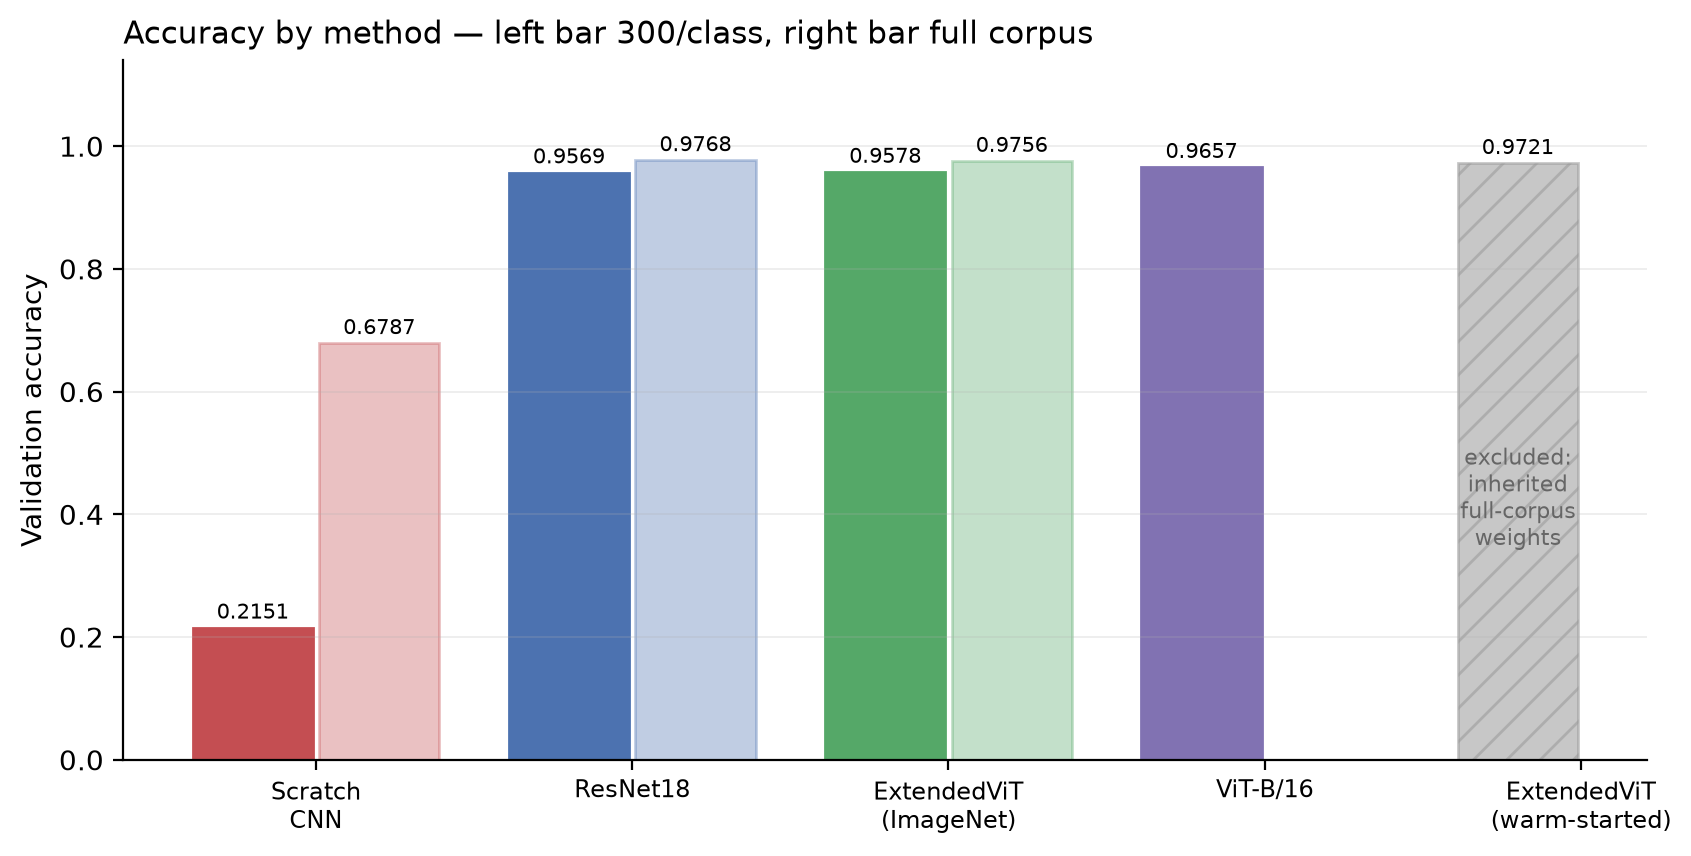
\includegraphics[width=0.85\linewidth]{fig7_results.png}
\caption{Accuracy by method: 300 images per class (left bar)
and the full corpus (right). The warm-started run is hatched and
excluded.}
\end{figure}

The scratch CNN's 0.2115 against its 0.6786 on the full corpus, a
46-point swing from data volume alone versus roughly 2 points for the
pretrained models, is the largest data-efficiency effect in the
study, and it belongs to the baseline rather than to the hybrid.

Figure 7 gives validation accuracy and loss per epoch; the inset resolves the three pretrained models, which are otherwise indistinguishable against the scratch CNN's trajectory. The ExtendedViT curve is the warm-started run excluded from Table 6 (final 0.972), so its lead from the first epoch reflects inherited weights rather than architecture (Section 4.9); The ResNet18 curve is the clean ImageNet-only rerun, as is ViT-B/16.

\begin{figure}
\centering
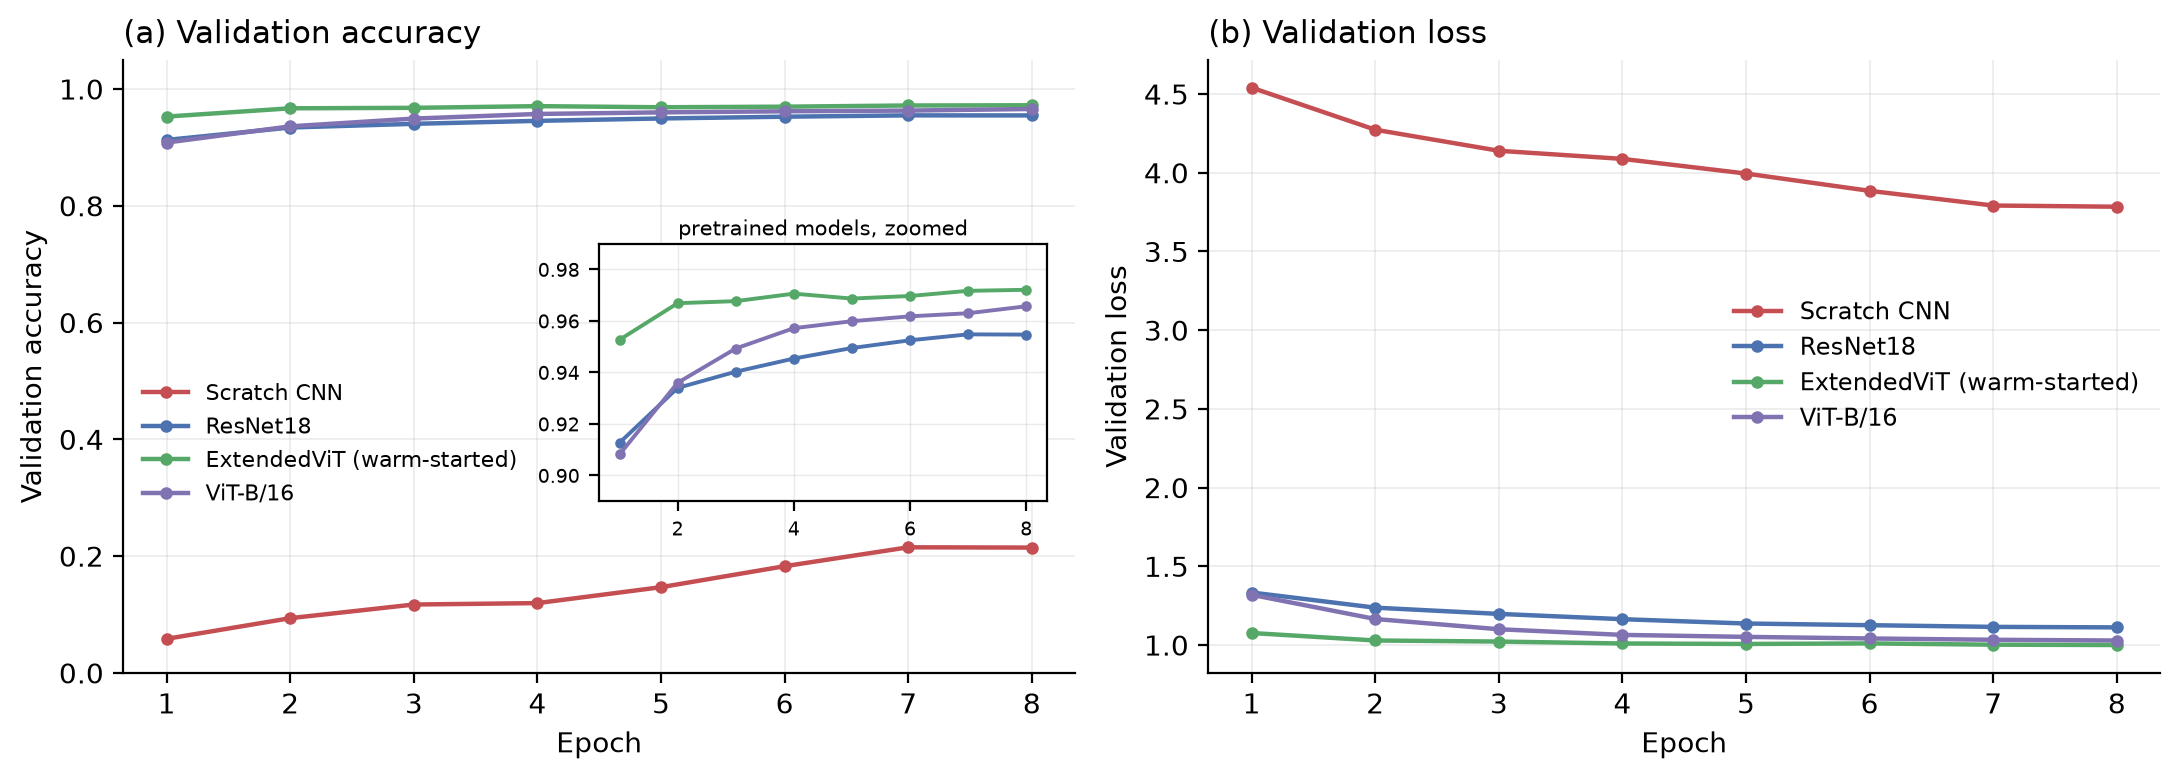
\includegraphics[width=0.85\linewidth]{fig6_training_curves.png}
\caption{Validation accuracy and loss per epoch at the
equal-budget setting; inset resolves the three pretrained models. ExtendedViT is the warm-started run; ResNet18 and ViT-B/16 are ImageNet-initialised (Section 4.3).}
\end{figure}

\hypertarget{controlled-budget-sweep-no-accuracy-advantage}{%
\subsection{Controlled Budget Sweep: No Accuracy
Advantage}\label{controlled-budget-sweep-no-accuracy-advantage}}

Tables 5 and 6 differ in source composition as well as size, and Table 5
carries an inherited initialisation, so neither isolates data volume.
The Ekush-only sweep does. Figure 8 plots the outcome; Table 7
gives the numbers, with 50 and 100 per class averaged over three seeds
and reported as mean ± standard deviation (standard error for the difference).

\begin{figure}
\centering
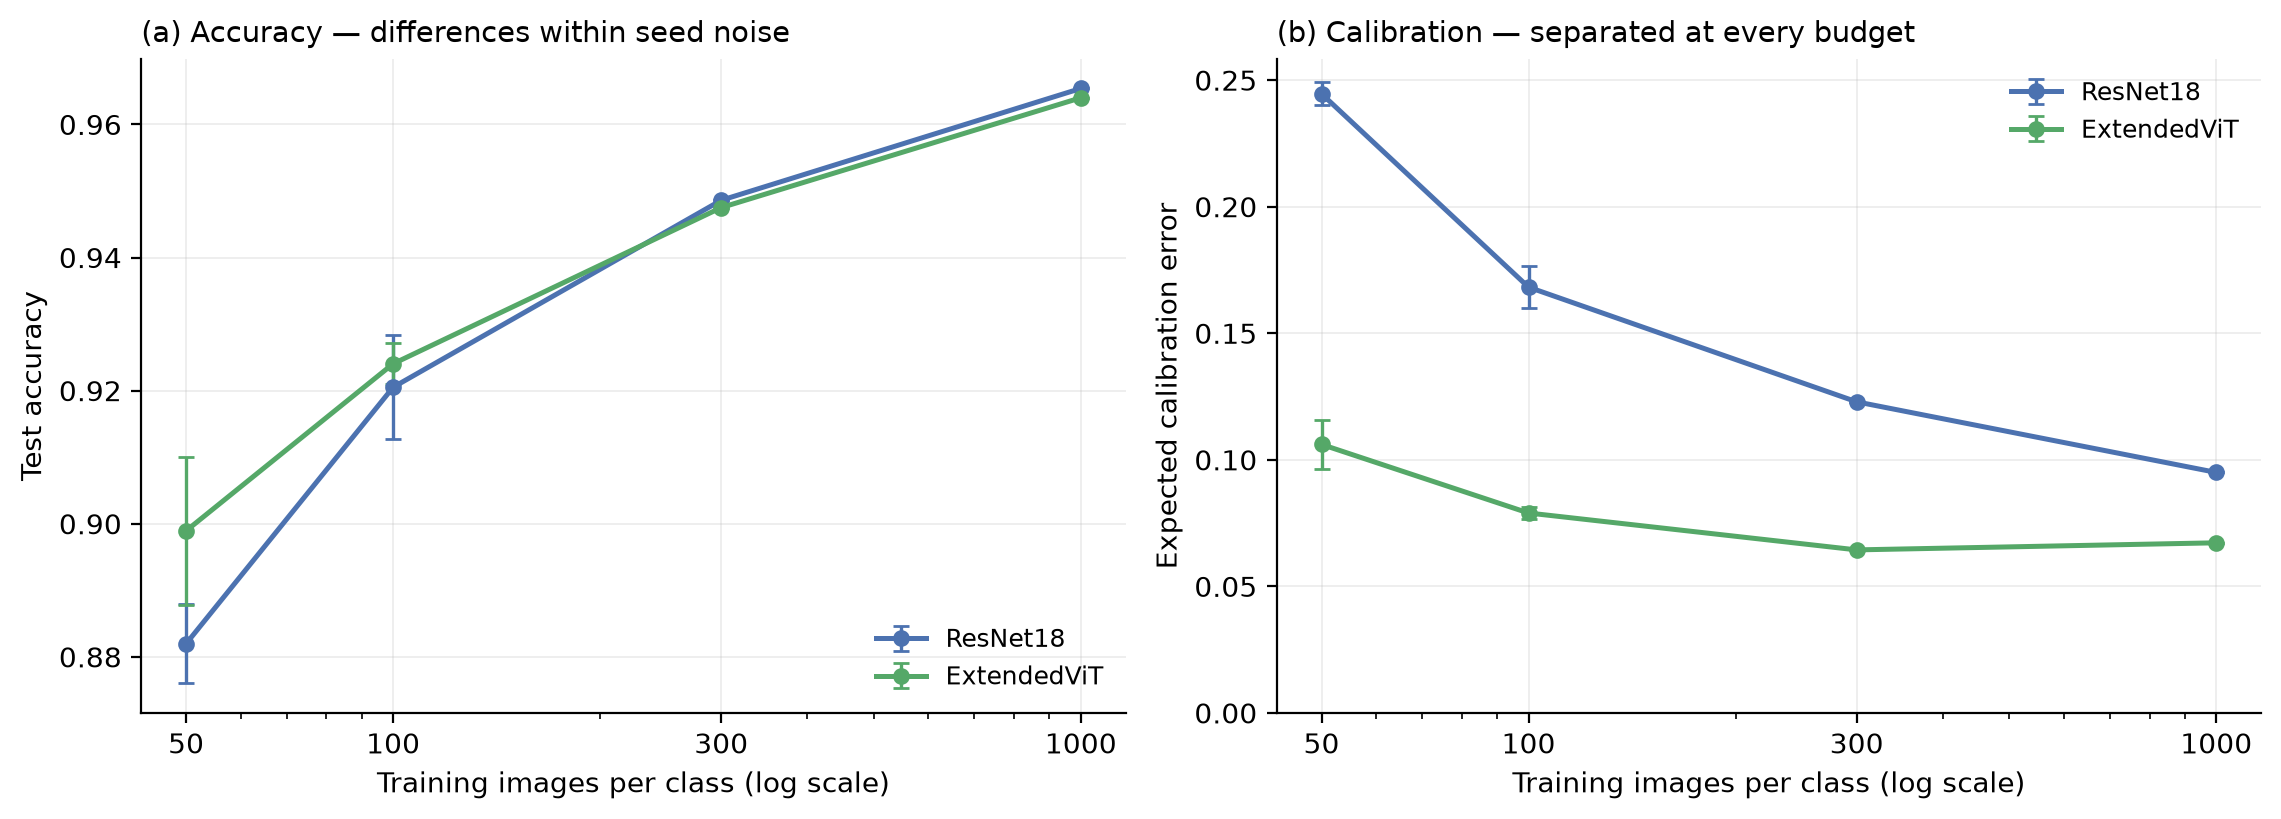
\includegraphics[width=0.85\linewidth]{fig10_data_efficiency_sweep.png}
\caption{Ekush-only budget sweep, ImageNet init throughout.
(a) Accuracy differences fall within seed noise. (b) Calibration error
before temperature scaling.}
\end{figure}

\begin{table*}[htbp]
\centering
\footnotesize
\caption{Ekush-only sweep (122 classes, ImageNet init
throughout). Accuracy in points; ResNet18 and ExtendedViT columns are mean ± s.d.\ over three seeds, Difference is mean ± standard error, and t is Welch's t.}
\begin{tabular}{rrrrr}
\toprule
Images/class & ResNet18 & Extended\-Vi\-T & Difference & t \\
\midrule
50 & 88.20 ± 0.59 & 89.89 ± 1.12 & +1.70 ± 0.73 & 2.33 \\
100 & 92.05 ± 0.78 & 92.40 ± 0.31 & +0.35 ± 0.49 & 0.73 \\
300 & 94.86 & 94.75 & −0.11 & --- \\
1000 & 96.54 & 96.40 & −0.14 & --- \\
\bottomrule
\end{tabular}
\end{table*}


\textbf{Significance.} No accuracy advantage survives. The largest difference, +1.70
points at 50 images per class, carries a standard error of 0.73 (Welch's t = 2.33, p \ensuremath{\approx} 0.10 with three seeds per model) and is not significant; ExtendedViT's own
seed-to-seed spread at that budget, ±1.12, exceeds the effect it would
demonstrate. At 100 the difference is +0.35 ± 0.49, and at 300 and 1,000
ResNet18 is fractionally ahead. A single-seed run at 50 per class
initially showed +2.46 points, which repetition reduced to +1.70, an
illustration of why single-seed differences at this magnitude should not
be reported as findings.

This paper therefore states plainly that the hypothesis motivating this study,
that a Transformer encoder atop a convolutional tokeniser generalises
more efficiently from few examples in top-1 terms, is \emph{not
supported}.

\hypertarget{calibration-and-why-it-is-not-an-architectural-advantage}{%
\subsection{Calibration, and Why It Is Not an Architectural
Advantage}\label{calibration-and-why-it-is-not-an-architectural-advantage}}

The same runs separate decisively on the quality of their probability
estimates (Table 8).

\begin{table*}[htbp]
\centering
\footnotesize
\caption{Expected calibration error, Ekush-only sweep (15 bins;
lower is better).}
\begin{tabular}{rrrrr}
\toprule
Images/class & ResNet18 & Extended\-Vi\-T & Ratio & t \\
\midrule
50 & 0.245 ± 0.005 & \textbf{0.106 ± 0.010} & 2.31× & 22.4 \\
100 & 0.168 ± 0.008 & \textbf{0.079 ± 0.002} & 2.13× & 17.7 \\
300 & 0.123 & \textbf{0.064} & 1.91× & --- \\
1000 & 0.095 & \textbf{0.067} & 1.41× & --- \\
\bottomrule
\end{tabular}
\end{table*}


ExtendedViT roughly halves ResNet18's calibration error at 50, 100 and 300
images per class, and cuts it by about a third at 1,000. The separation is large relative to seed variance (t
\textgreater{} 17 at both replicated budgets, with non-overlapping
ranges), and the ratio narrows monotonically as data grows (2.31×,
2.13×, 1.91×, 1.41×), the shape expected of an effect that compensates
for limited data. Negative log-likelihood follows the same pattern
(ExtendedViT 0.498 vs ResNet18 0.717 at 50 per class; 0.234 vs 0.240 at 1,000).

The mechanism is visible in mean predicted confidence. In one run at 50 images per class, ResNet18 averages 0.638 confidence against 0.887 accuracy, a
25-point under-confidence gap; ExtendedViT averages 0.794 against 0.911,
a 12-point gap. Both are under-confident: label smoothing of 0.1 caps
attainable confidence, and this inflates the absolute ECE of both models,
but ResNet18 markedly more so. Since both models train with
identical smoothing, the comparison is unaffected; absolute values
should not be compared against ECE figures from studies that omit
smoothing.

The encoder is therefore not finding additional correct answers. It is
producing sharper, better calibrated probability estimates from the same
evidence, which raises the question of whether the architecture is
required to obtain them.

The architecture is not required to obtain them. Temperature scaling \citep{ref48} is the standard
post-hoc calibration correction: divide the logits by a single scalar
fitted by minimising validation NLL, leaving accuracy exactly unchanged.
Applying it to both models dissolves the gap (Table 9).

\begin{table*}[htbp]
\centering
\footnotesize
\caption{Temperature scaling, Ekush-only sweep. Accuracy is unchanged by construction. Values come from the temperature-scaling runs and therefore differ slightly from the three-seed means in Table 8.}
\begin{tabular}{rlrrrrr}
\toprule
Budget & Model & T & ECE raw & ECE scaled & NLL raw & NLL scaled \\
\midrule
50/class & ResNet18 & 0.552 & 0.2496 & \textbf{0.0250} & 0.7174 &
0.4697 \\
50/class & Extended\-Vi\-T & 0.749 & 0.1171 & 0.0341 & 0.4985 & 0.4225 \\
100/class & ResNet18 & 0.628 & 0.1773 & 0.0232 & 0.4870 &
0.3338 \\
100/class & Extended\-Vi\-T & 0.787 & 0.0818 & \textbf{0.0152} & 0.3887 & 0.3285 \\
\bottomrule
\end{tabular}
\end{table*}


At 50 images per class a temperature-scaled ResNet18 (0.0250) is
\emph{better calibrated than an unscaled ExtendedViT} (0.1171, and
0.0341 once itself scaled). The fitted temperatures are below 1 for both
models, confirming that both were under-confident, an expected
consequence of the label smoothing used throughout, with ResNet18
simply further from calibrated than the hybrid.

The encoder was therefore compensating for a defect that one scalar
removes more cheaply and more completely. This paper concludes that the
calibration difference is not an architectural advantage. It is a
difference in how far each architecture's raw confidences sit from their
empirical accuracy under label smoothing, and it is fully correctable
post hoc. Reporting it as an architectural property, as the authors were
prepared to do before running this control, would have been wrong.

The broader methodological point generalises beyond this paper:
uncorrected ECE comparisons between architectures measure the
interaction between an architecture and a training recipe, not a
property of the architecture. Any calibration comparison should report
temperature-scaled figures alongside raw ones.

\hypertarget{cross-corpus-generalisation}{%
\subsection{Cross-Corpus
Generalisation}\label{cross-corpus-generalisation}}

A within-corpus split measures whether a model learned the characters;
it does not measure whether it learned them independently of how a
particular project collected its images. Since merging corpora
implicitly promises the latter, this study tests it directly: models are trained on one corpus and evaluated on another, restricted to the classes the two share so
the label space is identical on both sides. The only thing that changes
between training and test is the collection convention: resolution,
ink polarity, and writing population.

RAS-Compound and MatriVasha share 58 classes; RAS-Compound and Ekush
share 37. Ekush and MatriVasha share only 8, too few to be informative,
so that pair is omitted. Backbones are ImageNet-initialised only, since
a Bengali checkpoint would leak the target corpus into the source model.

\begin{table*}[htbp]
\centering
\footnotesize
\caption{Cross-corpus generalisation (300 images per class,
shared classes only).}
\begin{tabular}{>{\raggedright\arraybackslash}p{(\linewidth - 12\tabcolsep) * \real{0.1154}}
  >{\raggedright\arraybackslash}p{(\linewidth - 12\tabcolsep) * \real{0.1154}}
  >{\raggedleft\arraybackslash}p{(\linewidth - 12\tabcolsep) * \real{0.1538}}
  >{\raggedleft\arraybackslash}p{(\linewidth - 12\tabcolsep) * \real{0.1538}}
  >{\raggedleft\arraybackslash}p{(\linewidth - 12\tabcolsep) * \real{0.1538}}
  >{\raggedleft\arraybackslash}p{(\linewidth - 12\tabcolsep) * \real{0.1538}}
  >{\raggedleft\arraybackslash}p{(\linewidth - 12\tabcolsep) * \real{0.1538}}}
\toprule
\begin{minipage}[b]{\linewidth}\raggedright
Architecture
\end{minipage} & \begin{minipage}[b]{\linewidth}\raggedright
Train \ensuremath{\rightarrow} Test
\end{minipage} & \begin{minipage}[b]{\linewidth}\raggedleft
Shared
\end{minipage} & \begin{minipage}[b]{\linewidth}\raggedleft
Same-corpus val
\end{minipage} & \begin{minipage}[b]{\linewidth}\raggedleft
Cross-corpus test
\end{minipage} & \begin{minipage}[b]{\linewidth}\raggedleft
Chance
\end{minipage} & \begin{minipage}[b]{\linewidth}\raggedleft
Gap
\end{minipage} \\
\midrule
ResNet18 & Matri\-Vasha \ensuremath{\rightarrow} RAS & 58 & 0.9678 & 0.0317 & 0.017 & 0.936 \\
Extended\-Vi\-T & Matri\-Vasha \ensuremath{\rightarrow} RAS & 58 & 0.9632 & 0.0375 & 0.017 & 0.926 \\
ResNet18 & RAS \ensuremath{\rightarrow} Matri\-Vasha & 58 & 0.9915 & 0.0268 & 0.017 & 0.965 \\
Extended\-Vi\-T & RAS \ensuremath{\rightarrow} Matri\-Vasha & 58 & 0.9887 & 0.0254 & 0.017 & 0.963 \\
ResNet18 & Ekush \ensuremath{\rightarrow} RAS & 37 & 0.9658 & 0.0514 & 0.027 & 0.914 \\
Extended\-Vi\-T & Ekush \ensuremath{\rightarrow} RAS & 37 & 0.9604 & 0.0547 & 0.027 & 0.906 \\
ResNet18 & RAS \ensuremath{\rightarrow} Ekush & 37 & 1.0000 & 0.0418 & 0.027 & 0.958 \\
Extended\-Vi\-T & RAS \ensuremath{\rightarrow} Ekush & 37 & 1.0000 & 0.0205 & 0.027 & 0.980 \\
\bottomrule
\end{tabular}
\end{table*}


\textbf{Result.} Generalisation across corpora collapses to chance (Table 10). Every model
scores 0.96--1.00 on its own corpus's held-out split and 0.021--0.055 on
another corpus's images of \emph{the same characters}, between 0.8×
and 2.2× the chance rate of a 37- or 58-way classifier. The result holds
in both directions, for both architectures, and across both corpus
pairs. Figure 9 plots it.

\begin{figure}
\centering
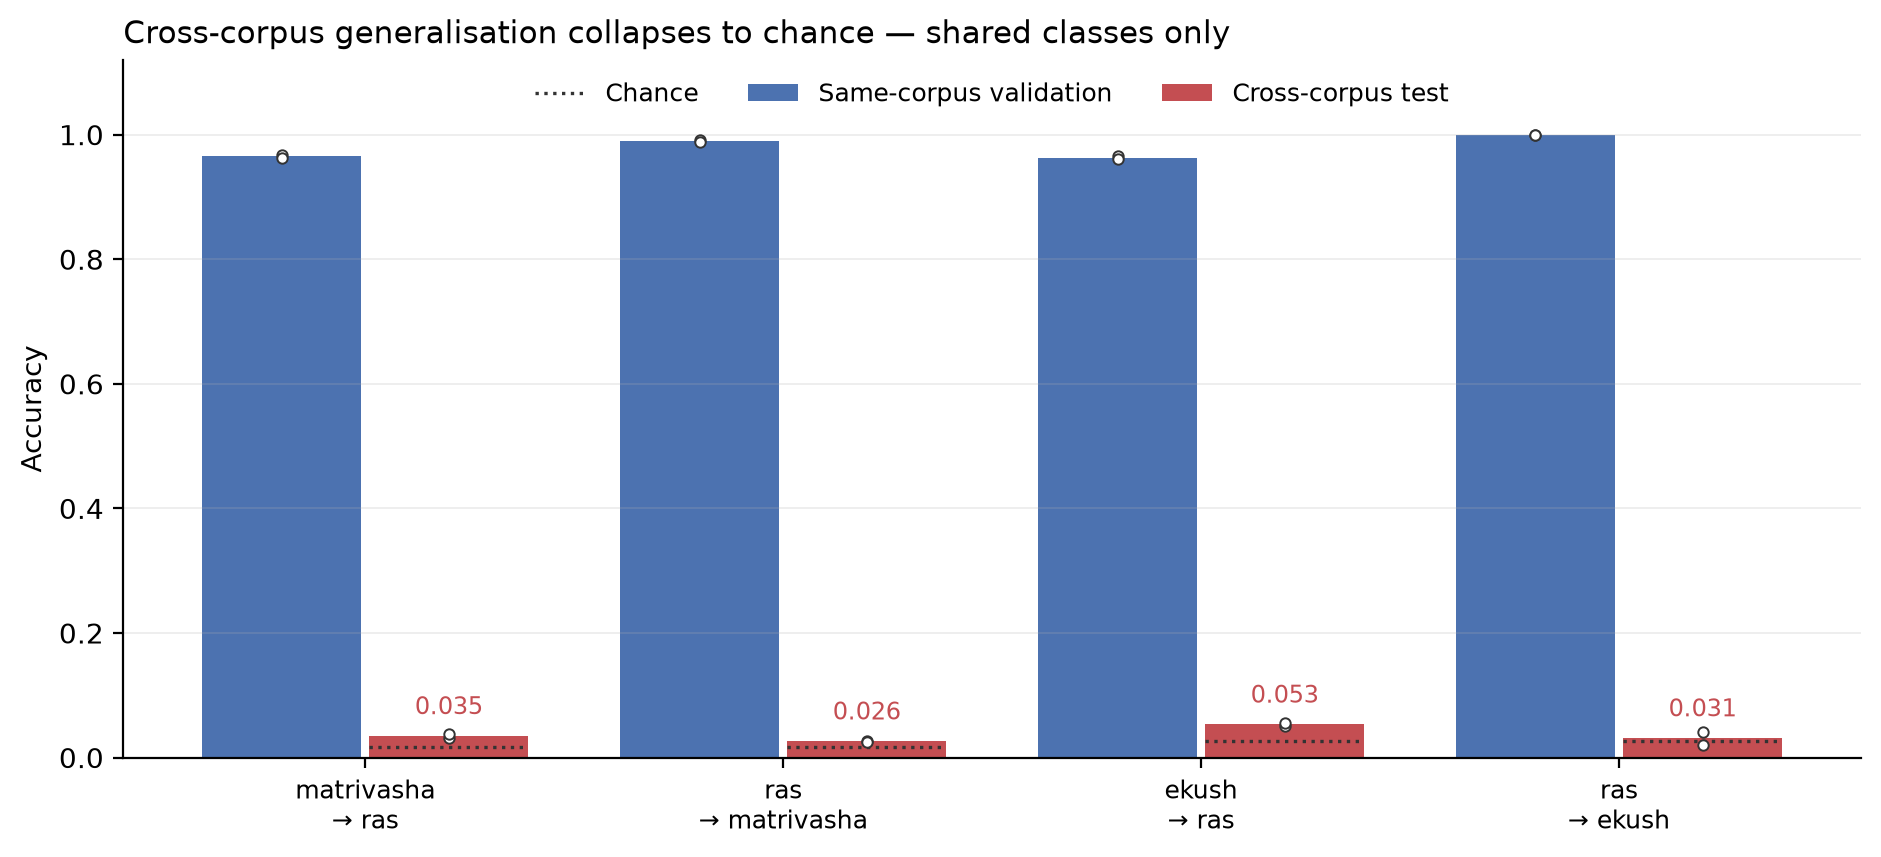
\includegraphics[width=0.85\linewidth]{fig11_cross_source.png}
\caption{Cross-corpus generalisation collapses to chance on
the classes each pair shares.}
\end{figure}

\textbf{Label consistency.} The collapse is not a labelling artifact. Near-chance transfer would
follow trivially if the corpora's class mappings disagreed, which would
also invalidate the merged benchmark. This was tested directly: the
merged full-corpus model classifies RAS-Compound's shared-class test
samples at 0.9921 and MatriVasha's at 0.9800. Both corpora's renderings
of a class map to the same label correctly, so the grapheme-level
reconciliation of Section 3.2 is sound and the collapse reflects genuine
domain shift.

\textbf{Interpretation.} A model trained on a single Bengali corpus
learns that corpus's rendering of compound characters: its resolution,
binarisation, ink polarity, and writer population. The 97.6\%
achieved by the merged model across all three corpora is attainable only
because it saw all three in training. It is not evidence of a general
character recogniser, and neither, by extension, are the near-ceiling
accuracies the literature reports on individual corpora \citep{ref11,ref12,ref17,ref23}: those numbers describe within-corpus
competence and may substantially overstate performance on newly
collected handwriting.

The finding reframes what merging is for. Merging is usually motivated
as enlarging the training set; here it is better understood as
\emph{covering domains}, since no single corpus yields a model that
transfers to another. It also identifies the concrete gap the field
should target: domain-invariant representations for handwritten
Bengali, which the preprocessing of Section 3.3 evidently does not
achieve, despite normalising polarity and scale.

\textbf{Caveats.} Training was capped at 300 images per class; larger
budgets might narrow the gap, though the effect size makes it
implausible that they close it. The two RAS-trained rows reach 1.0000
same-corpus validation, which suggests unusually low intra-class
variation in that corpus and inflates the gap for those directions
specifically. And each pair is a single run, though the consistency
across eight runs and four directions makes seed variance an unlikely
explanation for an effect of this magnitude.

\hypertarget{inference-cost}{%
\subsection{Inference Cost}\label{inference-cost}}

Figure 10 plots accuracy against single-image CPU latency, measured on one thread of the Apple M4 CPU. ExtendedViT runs in 13 ms against ViT-B/16's 45
ms, 3.4× faster with 3.6× fewer parameters, because attention
operates over 50 tokens rather than 197. Relative to ResNet18's 11 ms,
the transformer encoder adds approximately 2.6 ms per image without an accuracy gain, and its raw calibration advantage is available to ResNet18 through temperature scaling at negligible cost (Section 4.5). For the resource-constrained deployment scenarios the literature emphasises \citep{ref18,ref20}, ResNet18 is therefore the more economical choice; ExtendedViT's case rests only on being 3.4× cheaper than ViT-B/16 for roughly one accuracy point less at the equal budget.

\begin{figure}
\centering
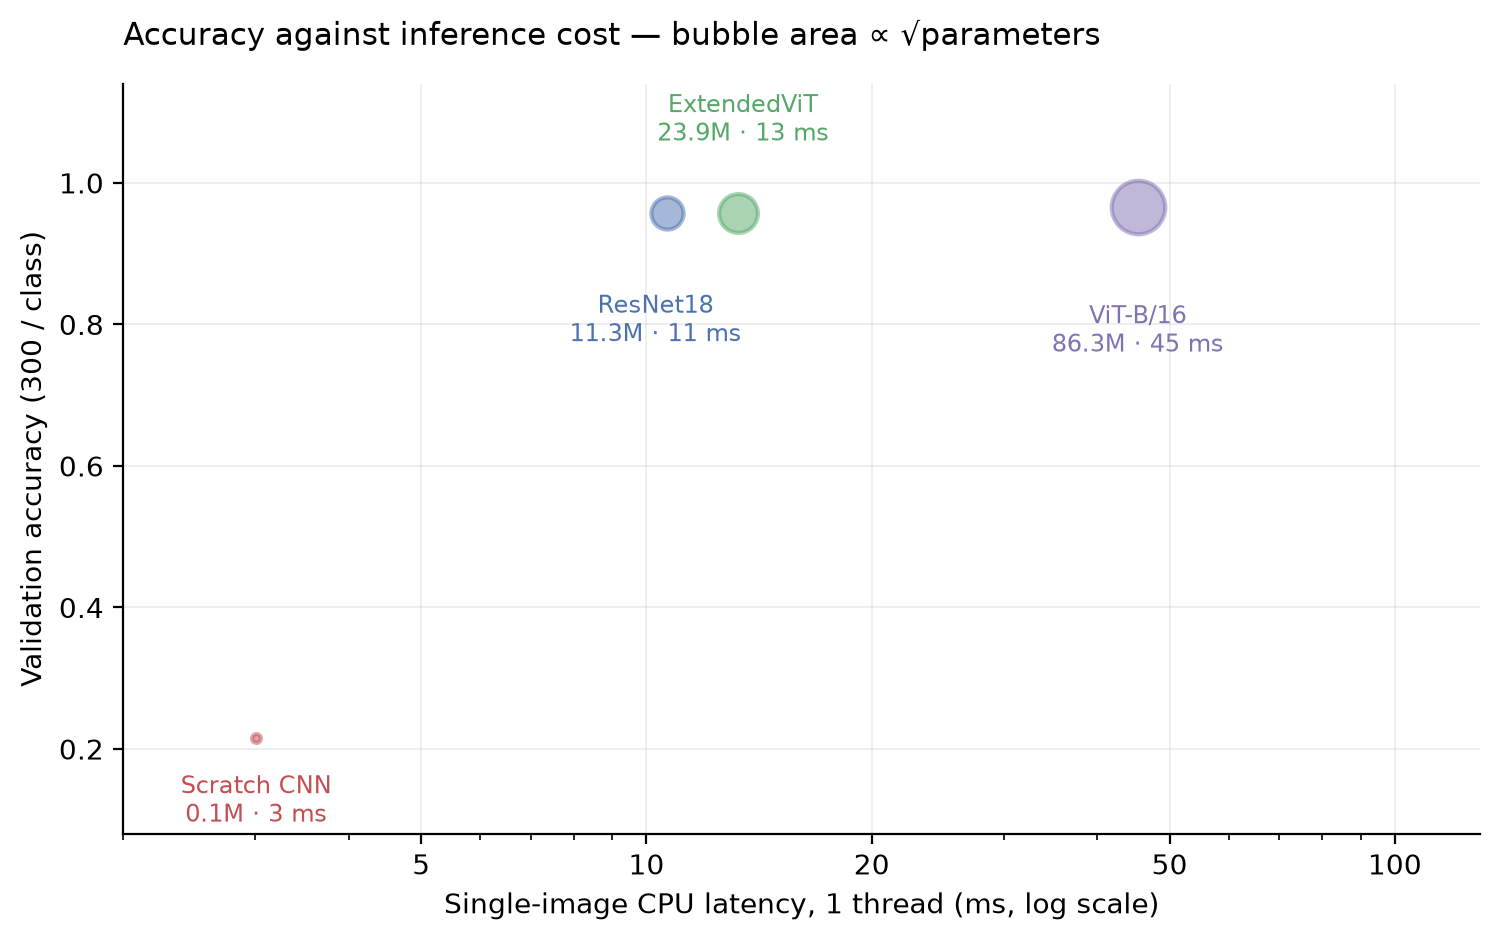
\includegraphics[width=0.85\linewidth]{fig9_efficiency.png}
\caption{Accuracy against single-image CPU latency; bubble
area is proportional to the square root of parameter count.}
\end{figure}

\hypertarget{attention-analysis}{%
\subsection{Attention Analysis}\label{attention-analysis}}

Figure 11 visualises the classification token's attention over
the 7×7 token grid in the final encoder layer, upsampled and overlaid on
the input glyph. A consistent pattern emerges: attention concentrates on the conjunct body and systematically avoids the head-line. This is plausible behaviour: the head-line is present in nearly every Bengali character and carries little class-discriminative information, while the structure of the conjoined consonant forms beneath it carries most of it. The maps show that the encoder attends to sensible regions without supervision directing it to do so; they do not show that attention is needed to exploit those regions, since ResNet18 reaches the same accuracy without it (Sections 4.2 and 4.4).

\begin{figure}
\centering
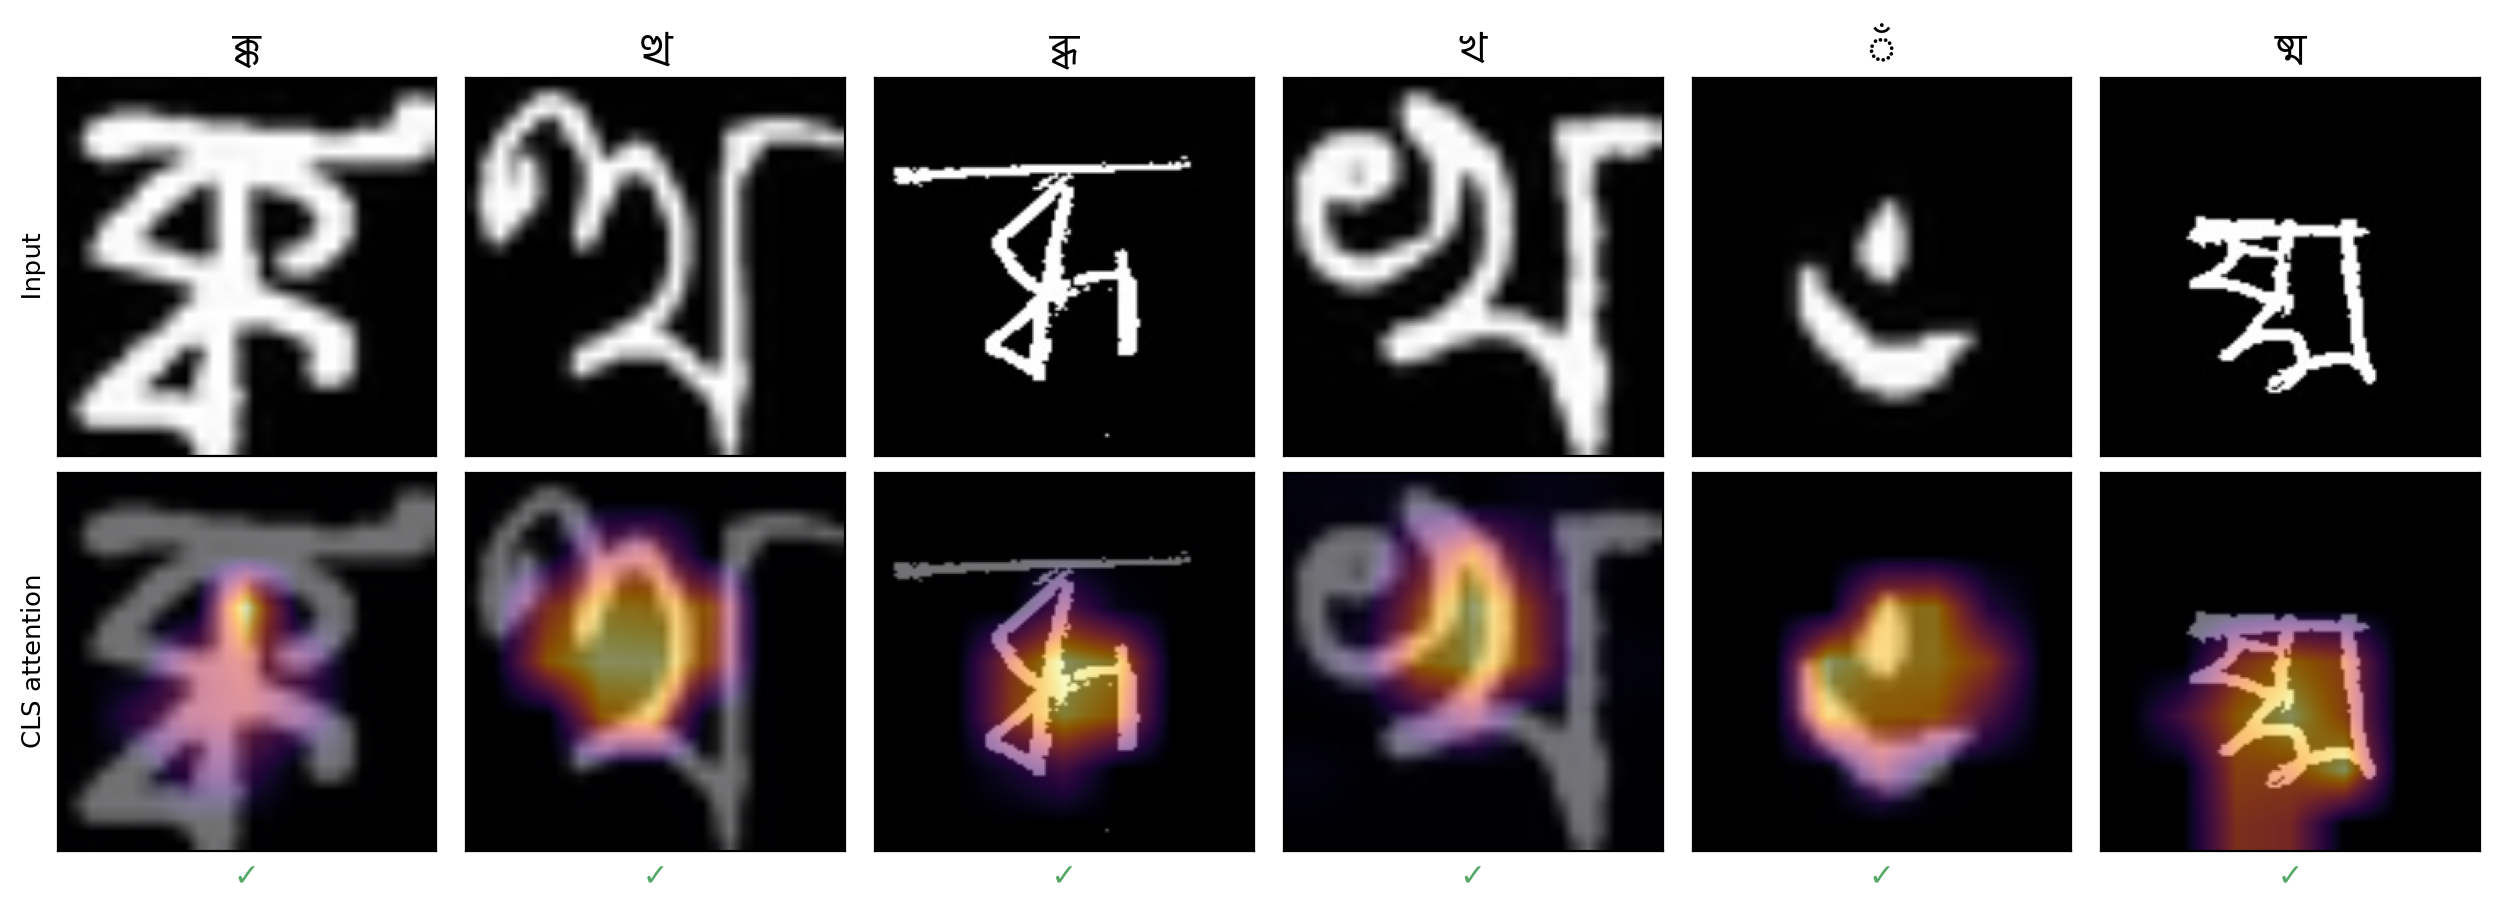
\includegraphics[width=0.85\linewidth]{fig8_attention.png}
\caption{Classification-token attention over the 7×7 token
grid, overlaid on the input glyph. Attention avoids the shared matra
head-line.}
\end{figure}

Attention weights are extracted by running the encoder stack manually
rather than through \texttt{nn.TransformerEncoder}; the manual pass is
asserted to reproduce the model's own logits, which also serves as a
check on the formulation given in Section 3.4.

\hypertarget{ablation-studies}{%
\subsection{Ablation Studies}\label{ablation-studies}}

\textbf{Backbone initialisation.} Holding everything else fixed,
initialising ExtendedViT's trunk from ImageNet rather than from the
full-corpus ResNet18 checkpoint costs 1.43 accuracy points at the
equal-budget setting (0.9719 \ensuremath{\rightarrow} 0.9576). The inherited trunk had seen the
entire corpus, so that 1.43-point difference measures leaked information
rather than architecture. The equivalent inheritance in ResNet18,
from a RAS-only checkpoint, changed its equal-budget accuracy by only 0.15
points (0.9544 inherited, 0.9529 from ImageNet alone; Section 4.3).
Sections 4.4 and 4.5
use ImageNet initialisation throughout for both architectures.

\textbf{Temperature scaling.} As reported in Section 4.5, a single
scalar fitted on validation data removes the calibration difference
between architectures entirely. This was the decisive control for the
paper's remaining architectural claim, and it did not survive it.

\hypertarget{comparison-with-prior-published-results}{%
\subsection{Comparison with Prior Published
Results}\label{comparison-with-prior-published-results}}

\begin{table*}[htbp]
\centering
\footnotesize
\caption{Positioning against prior Bengali character recognition
work.}
\begin{tabular}{>{\raggedright\arraybackslash}p{(\linewidth - 8\tabcolsep) * \real{0.1765}}
  >{\raggedright\arraybackslash}p{(\linewidth - 8\tabcolsep) * \real{0.1765}}
  >{\raggedright\arraybackslash}p{(\linewidth - 8\tabcolsep) * \real{0.1765}}
  >{\raggedleft\arraybackslash}p{(\linewidth - 8\tabcolsep) * \real{0.2353}}
  >{\raggedleft\arraybackslash}p{(\linewidth - 8\tabcolsep) * \real{0.2353}}}
\toprule
\begin{minipage}[b]{\linewidth}\raggedright
Study
\end{minipage} & \begin{minipage}[b]{\linewidth}\raggedright
Architecture
\end{minipage} & \begin{minipage}[b]{\linewidth}\raggedright
Dataset
\end{minipage} & \begin{minipage}[b]{\linewidth}\raggedleft
Classes
\end{minipage} & \begin{minipage}[b]{\linewidth}\raggedleft
Reported
\end{minipage} \\
\midrule
Das et al.~\citeyearpar{ref3} & Convex-hull + quad-tree + SVM & CMATERdb
3.1.3.3 & 171 & 79.35\% \\
Roy et al.~\citeyearpar{ref9} & Layer-wise DCNN & CMATERdb 3.1.3.3 & 171 &
90.33\% \\
Chatterjee et al.~\citeyearpar{ref11} & ResNet-50, ImageNet &
Bangla\-Lekha-Isolated & 84 & 96.12\% \\
Ghosh et al.~\citeyearpar{ref12} & Inception\-Res\-Net\-V\-2 / Dense\-Net\-121 &
CMATERdb & 231 & 96.99\% \\
Compound\-Dense\-Net \citep{ref23} & Modified DenseNet & Bangla\-Lekha / Ekush /
CMATERdb & varies & 96.2--98.5\% \\
Parvez et al.~\citeyearpar{ref17} & ViT-B/16 & CMATERdb 3.1.2 (basic) & 50 &
98.26\% \\
ResViT \citep{ref19} & Res\-Net\-50v\-2 + ViT, parallel fusion &
Bangla\-Lekha-Isolated & 84 & 97.21\% \\
Raquib et al.~\citeyearpar{ref25} & Efficient\-Net\-B\-3 + ViT + Conformer & Own
(78-class) / CHBCR & 78 & 98.84\% / 96.49\% \\
\textbf{This work} & \textbf{ResNet18 tokeniser + Transformer encoder} &
\textbf{Unified RAS + Ekush + MatriVasha} & \textbf{256} &
\textbf{97.60\%} (full corpus) \\
\bottomrule
\end{tabular}
\end{table*}


\textbf{Comparability.} Table 11 sets the result against prior work. These numbers are not a leaderboard and must not be presented as one. Class counts range from 50 to 256, evaluation protocols and splits
differ, several sets are near-balanced while the corpus used here is deliberately not,
and some reported figures are averages over balanced subsets. A 98.26\%
on 50 basic characters \citep{ref17} is a substantially easier problem than
97.60\% on 256 classes including the full compound inventory and a
27-class rare tail. The table's purpose is to show that the result reported here sits
in the range established by recent deep architectures while being
obtained on a markedly larger and more imbalanced label space, not to
claim state of the art.

\hypertarget{per-source-and-per-class-analysis}{%
\subsection{Per-Source and Per-Class
Analysis}\label{per-source-and-per-class-analysis}}

Per-source accuracy is reported in Table 5. Both pretrained models run on the full corpus score highest on RAS-Compound (0.991--0.994) and lowest on Ekush
(0.974), the reverse of what corpus size alone would predict:
RAS-Compound is the smallest source but has the cleanest,
highest-resolution binarised glyphs, while Ekush is natively 28×28.
Image quality dominates corpus size here. The scratch CNN inverts this
completely (0.013 on RAS-Compound, 0.707 on Ekush), because without a
pretrained prior it learns only what it sees in quantity.

\textbf{Rare classes.} The rarest classes are the easiest, not the hardest. The 27 classes
with fewer than 100 images reach a mean per-class F1 of 0.9966
(ExtendedViT; 0.9925 for ResNet18) against 0.9758 for the 229
well-populated classes. This inverts the
usual expectation and follows directly from the confound established in
Section 3.2: those 27 classes are contributed solely by RAS-Compound,
whose images are high-resolution and cleanly binarised, and no other
corpus supplies a competing rendering of them. Their scarcity is an
artifact of source size, while their separability comes from image
quality. On this benchmark, therefore, \emph{macro-F1 does not measure
long-tail performance}, and neither macro-F1 nor per-class accuracy
should be read as evidence about rare conjuncts. This paper reports macro-F1 as a
descriptive statistic only.

\textbf{Confusions.} Errors concentrate on minimally different conjunct pairs. Only
7 of 256 classes fall below F1 0.90 for ExtendedViT (6 for ResNet18). The most-confused pairs are
near-identical, and both architectures fail on essentially the same
ones (Table 12):

\begin{table*}[htbp]
\centering
\footnotesize
\caption{Most-confused class pairs, full corpus (Extended\-Vi\-T /
ResNet18 error counts).}
\begin{tabular}{lrrl}
\toprule
True \ensuremath{\rightarrow} Predicted & Extended\-Vi\-T & ResNet18 & What differs \\
\midrule
\bn{ন্ড্র} \ensuremath{\rightarrow} \bn{ণ্ড্র} & 33 & 25 & dental \bn{ন} vs retroflex \bn{ণ} \\
\bn{ণ্ড্র} \ensuremath{\rightarrow} \bn{ন্ড্র} & 24 & 28 & the same pair, reversed \\
\bn{ম্ভ্র} \ensuremath{\rightarrow} \bn{ন্ত্র} & 32 & 26 & both components \\
\bn{ত্ত} \ensuremath{\rightarrow} \bn{ও} & 25 & 26 & conjunct resembling a vowel \\
\bn{ম্ন} \ensuremath{\rightarrow} \bn{ম্ম} & 19 & 19 & \bn{ন} vs \bn{ম} as second component \\
\bn{ন্ঢ} \ensuremath{\rightarrow} \bn{ন্ট} & 15 & 16 & \bn{ঢ} vs \bn{ট} \\
\bn{শ্ন} \ensuremath{\rightarrow} \bn{শ্ম} & 12 & 13 & \bn{ন} vs \bn{ম} as second component \\
\bn{ন্ব} \ensuremath{\rightarrow} \bn{ণ্ব} & 12 & 12 & dental \bn{ন} vs retroflex \bn{ণ} \\
\bn{ত্থ} \ensuremath{\rightarrow} \bn{থ} & 12 & 11 & conjunct vs its own second component \\
\bn{২} \ensuremath{\rightarrow} \bn{হ} & 13 & 13 & digit against a consonant \\
\bottomrule
\end{tabular}
\end{table*}


Three systematic patterns emerge. First, the \emph{dental/retroflex
nasal contrast} (\bn{ন} vs \bn{ণ}) accounts for the single largest error source,
and it is symmetric: the confusion runs in both directions,
indicating genuine visual ambiguity rather than a class prior. The
worst-performing classes overall are exactly this pair, \bn{ন্ড্র} (F1
0.8652 for ExtendedViT) and \bn{ণ্ড্র} (F1 0.8781), the two halves of the same confusion.
Second,
\emph{\bn{ন} vs \bn{ম} as a second component} recurs across otherwise unrelated
conjuncts. Third, conjuncts are confused with \emph{their own
constituents} (\bn{ত্থ} \ensuremath{\rightarrow} \bn{থ}) or with visually similar non-conjuncts (\bn{ত্ত} \ensuremath{\rightarrow} \bn{ও}, \bn{২}
\ensuremath{\rightarrow} \bn{হ}), which is a failure of compositional structure rather than of
stroke detection.

That both architectures fail on the same pairs, in similar proportions,
indicates these errors are properties of the data rather than of the
model, consistent with the near-identical aggregate accuracies of
Table 5, and with the inter-class similarity the literature identifies
as the field's persistent obstacle \citep{ref17,ref23,ref32}. Full
per-class results are in Appendix C; confusion matrices are
supplementary material.


\hypertarget{discussion}{%
\section{Discussion}\label{discussion}}

\textbf{Corpus versus architecture.} The corpus matters far more than the architecture.
Section 4.6 sets the scale for the architecture comparison. Every
difference between architectures reported in this paper is at most a few
accuracy points; the difference between evaluating within a corpus and
across corpora is ninety. Any conclusion about which architecture is
best for Bengali compound characters is therefore conditional on a fixed
collection convention, and would need re-establishing on data collected
differently. This comes before the architecture results because it limits
how much weight they can carry.

\textbf{Accuracy.} This study set out expecting the hybrid to be more accurate than a convolutional baseline
when data is limited. That expectation was not met. Across a controlled sweep with the sole
variable being per-class budget, and with three seeds at the two
smallest budgets, no accuracy difference reaches significance; at the
two largest budgets ResNet18 is fractionally ahead. The alternative,
presenting the single-seed +2.46 points at 50 images per class or the
1.75-point margin from the contaminated warm-started run, would have
reported a finding that disappears under repetition and a proper control.

\textbf{Calibration.} The encoder yields better-calibrated raw probabilities: roughly half ResNet18's expected calibration error at every budget, largest when data is scarcest and narrowing monotonically as data grows, with a separation an order of magnitude larger than seed variance. That difference is not architectural. A single temperature fitted on validation data removes it (Section 4.5), and a temperature-scaled ResNet18 is better calibrated than an unscaled ExtendedViT. The two architectures sit at different distances from calibration under the shared training recipe; attention does not confer better-calibrated posteriors that post-hoc scaling cannot supply.

Why the raw gap arises is not established here. Both models are under-confident under label smoothing of 0.1, ResNet18 more so (0.638 mean confidence at 0.887 accuracy in one run at 50 images per class), and the fitted temperatures (0.552 against 0.749) quantify that difference. Whether it reflects the encoder's aggregation over the whole glyph or only a different interaction between each architecture and label smoothing would require a replication without smoothing; the attention maps of Section 4.8 are compatible with either account.

\textbf{Relevance of calibration.} Isolated-character accuracy is
rarely the end goal. In word- and line-level recognition the character
posterior feeds a decoder (beam search, a language model, or a
lexicon-constrained search) which consumes probabilities rather than argmax labels. For Bengali, where conjuncts are mutually confusable and a decoder must arbitrate between close alternatives, the shape of the posterior is arguably more consequential than its mode. The results here imply that this requirement is met more cheaply by post-hoc temperature scaling than by architectural choice: a scaled ResNet18 supplies a posterior comparably calibrated to the hybrid's, at lower latency.

\textbf{Relation to prior work.} That ViT-B/16 leads the properly
initialised equal-budget comparison (Table 6) reproduces, on compound
characters and a 256-class label space, the ordering Parvez et
al.~\citeyearpar{ref17} reported for basic characters. This paper quantifies the cost of
that finding: ViT-B/16
buys roughly one accuracy point over ExtendedViT at 3.6× the parameters
and 3.4× the inference time. Numbers are not directly comparable across
studies given differing class counts and protocols, but for orientation
ResViT reports 97.21\% on BanglaLekha-Isolated \citep{ref19} and
CompoundDenseNet 96.2--98.5\% across three benchmarks \citep{ref23}, both on
smaller class inventories than the 256 used here.

\textbf{Threats to validity.}

\emph{Initialisation contamination.} Both pretrained models initially inherited previously trained Bengali weights (ResNet18 from a
RAS-only checkpoint, ExtendedViT from the full-corpus ResNet18), which
invalidated the first equal-budget comparison. Removing that inheritance
lowers ExtendedViT's first-epoch validation accuracy from 0.953 to 0.867. Every number
in Sections 4.4 and 4.5 comes from runs initialised from ImageNet alone.
Table 5 retains the inherited initialisation for ResNet18 and is
annotated accordingly; it should be read as an upper bound for that
baseline rather than as a controlled comparison. The equal-budget
ResNet18 result in Table 6 was rerun from ImageNet alone (Section 4.3).

\emph{Seeds and statistical power.} Three seeds establish that the
accuracy differences are not significant and that the calibration
differences are, but three is a small sample; the 300 and 1,000
per-class budgets are single runs, so their calibration figures carry no
error estimate.

\emph{Calibration measurement.} Label smoothing of 0.1 depresses
attainable confidence and inflates the absolute ECE of both models
\citep{ref56}. The
comparison is unaffected because smoothing is identical, but the
absolute ECE values reported here should not be compared against studies that omit it,
and a replication without smoothing would strengthen the claim.

\emph{Epoch budget.} All models train for 8 epochs, which suits
fine-tuning but may underserve the scratch CNN, whose 0.2115 should be
read as its 8-epoch result at that budget rather than a ceiling.

\textbf{Limitations.} Evaluation is on isolated characters; performance
within connected words, where segmentation error compounds
classification error, is not measured, and it is precisely there that calibration, raw or temperature-scaled, would have to be shown to matter practically. The sweep uses one corpus, so whether the calibration
effect generalises across image conventions is untested. The corpora may
not represent natural document imagery. And because class rarity is
perfectly confounded with source identity (Section 3.2), no
claim is made about rare-class behaviour. Architectural ablations (encoder depth, including
$L = 0$, head count, positional embeddings, polarity normalisation, and
backbone depth) were not run. Finally, the split is stratified by class but not by writer, so within-corpus test sets may contain writers seen in training, which would inflate within-corpus accuracy and therefore overstate the cross-corpus gap.


\hypertarget{conclusion}{%
\section{Conclusion}\label{conclusion}}

This study unified three Bengali handwriting corpora into a 256-class,
681,309-image benchmark by reconciling labels at the level of
Unicode-normalised graphemes, and used it to evaluate four architectures
under an identical protocol.

The benchmark's main finding is negative: trained on one constituent corpus and
tested on another, every architecture falls from 0.96--1.00 same-corpus
accuracy to 0.02--0.05 cross-corpus, verified as domain shift rather
than label disagreement (Section 4.6). A model trained on one Bengali
corpus therefore learns only that corpus's rendering of compound
characters, and single-corpus accuracies, including the near-ceiling figures widely
reported in this literature, should not be read as evidence of
generalisation. Merging corpora adds domain coverage.

Against that backdrop, architecture differences are small. The three pretrained architectures, spanning 11.3M to 86.3M parameters, differ by less than two accuracy points once initialisation is controlled, and only the from-scratch CNN falls far behind. The hybrid's
apparent calibration advantage is fully correctable by temperature
scaling, a property of the training recipe rather than the
architecture. ViT-B/16 is the most accurate model at an equal budget, at
3.6× the parameters and 3.4× the inference cost of the hybrid.

Three methodological cautions follow, each discovered by attempting to
falsify a claim made in this paper: warm-starting from a previously
trained checkpoint, routine in this literature, inflated the
equal-budget result by 1.43 accuracy points; macro-F1 does not measure
long-tail performance on this corpus, since rarity is confounded with
source image quality; and architecture-level calibration comparisons
should always be reported temperature-scaled. Transfer learning also makes the minority corpus's 27
otherwise-unavailable classes learnable: without pretraining, a scratch CNN reaches
0.0129 accuracy on that corpus against 0.707 on the largest.

Future work follows directly from the cross-corpus result. The field
needs domain-invariant representations for handwritten Bengali, since
the preprocessing used here does not achieve them, and
held-out-corpus evaluation should become standard practice alongside
within-corpus splits. On the architecture side, these results suggest
the returns from further model design on isolated Bengali compound
characters are limited relative to the evaluation and data problems
above; where architecture does matter is cost, and establishing the
accuracy-per-millisecond frontier for CPU-only deployment remains open.


\hypertarget{reproducibility}{%
\section{Reproducibility}\label{reproducibility}}

All results are produced by a single codebase in which dataset scanning,
label reconciliation, splitting, and image transformation are shared
across architectures; only the model varies. The train/validation/test
partition is derived deterministically from a fixed seed (42) applied to
a per-class shuffle, so the partition is identical for every run
reported here and can be regenerated exactly.

\begin{table*}[htbp]
\centering
\footnotesize
\caption{Complete training configuration.}
\begin{tabular}{>{\raggedright\arraybackslash}p{(\linewidth - 2\tabcolsep) * \real{0.5000}}
  >{\raggedright\arraybackslash}p{(\linewidth - 2\tabcolsep) * \real{0.5000}}}
\toprule
\begin{minipage}[b]{\linewidth}\raggedright
Setting
\end{minipage} & \begin{minipage}[b]{\linewidth}\raggedright
Value
\end{minipage} \\
\midrule
Input resolution & 224 × 224, 3-channel grayscale \\
Batch size & 32 \\
Epochs & 8 \\
Optimiser & AdamW, weight decay 10⁻⁴ \\
Base learning rate & 10⁻³ (CNN), 3×10⁻⁴ (ResNet18, Extended\-Vi\-T), 10⁻⁴
(ViT-B/16) \\
Backbone learning rate & 0.1 × base for all pretrained models \\
Schedule & Cosine annealing to 10⁻⁶ over 8 epochs \\
Loss & Cross-entropy, label smoothing 0.1 \\
Gradient clipping & Max norm 1.0 \\
Augmentation & Rotation ±15°, translation $\leq$10\%, shear 5°,
brightness/contrast jitter 0.3 \\
Normalisation & μ = σ = 0.5 per channel \\
Model selection & Best validation accuracy \\
Split & 80/10/10 stratified per class, seed 42 \\
Framework & PyTorch 2.13, torchvision 0.28, timm 1.0.28 (ResNet18 rerun and latency: 2.14.1, 0.29.1, 1.0.30) \\
Hardware & Apple Mac mini (M4 chip), Metal Performance Shaders backend \\
Inference measurement & Apple M4 CPU, single image, one thread \\
\bottomrule
\end{tabular}
\end{table*}


Table 13 gives the complete training configuration, and Figure 12 lists the commands that reproduce every result.

\begin{figure*}[htbp]
\centering
\small
\begin{verbatim}
python train_arch.py \
    --arch {cnn,resnet18,vit,extended_vit} \
    [--limit-per-class 300] [--no-warm-start]
python evaluate.py [--limit-per-class 300] \
    [--suffix _imagenet] --confusion --per-class
python cross_source.py --train <corpus> \
    --test <corpus> --arch <arch>
python temperature_scaling.py --source ekush --limit-per-class 50
python paper/figures.py
\end{verbatim}
\caption{Commands to reproduce every result.}
\end{figure*}

Code, trained checkpoints, and the label-reconciliation mapping files
are available at the repository named in the Code Availability statement
below.


\hypertarget{declarations}{%
\section{Declarations}\label{declarations}}

\textbf{Funding.} The authors received no funding for this work.

\textbf{Competing interests.} The authors declare that they have no known competing financial interests or personal relationships that could have appeared to influence the work reported in this paper.

\textbf{Author contributions.} All authors contributed to software development, data curation and processing, model training and evaluation, validation (including cross-checking of reported numbers and references), and writing of the original draft.

\textbf{Ethics.} This study uses only previously published, publicly available datasets and involved no new data collection from human participants.

\textbf{Data availability.} The three source corpora are pre-existing
public datasets. Ekush \citep{ref29}, MatriVasha \citep{ref49}, and
RAS-Compound \citep{ref50} are each described in peer-reviewed
publications, in addition to RAS-Compound's own distribution as a
Kaggle dataset. Their distribution terms are governed by each source's
own licence; where the licence permits, the merged 256-class manifest
itself is released alongside the reconciliation code. The
label-reconciliation mapping files (\texttt{ras\_class\_mapping.csv},
\texttt{matrivasha\_mapping.csv}) and the manifest-construction code
that reproduces the unified corpus are released with this paper.

\textbf{Code availability.} The code, the label-reconciliation mapping files, and the unified manifest with its fixed split are available at \url{https://github.com/uthsobcb/bangla-hcr-benchmark} and archived on Zenodo (\url{https://doi.org/10.5281/zenodo.23220342}).

\textbf{Acknowledgements.} The authors thank the creators of
RAS-Compound, Ekush, and MatriVasha for releasing their data publicly,
without which this benchmark would not have been possible.

\textbf{Use of AI tools.} Generative AI (Claude, Anthropic) was used
during manuscript preparation to cross-check reported statistics against
the underlying experiment logs and result files, to merge and renumber
the literature review into the main text, to adapt the manuscript to the
journal template, and to copy-edit and reword prose for clarity and
register, including a pass to reduce repetitive phrasing. It was not used
to design experiments, run models, or generate results. The authors
reviewed and edited all AI-assisted text, verified all reported numbers
and citations against their own logged output and sources, and take full
responsibility for the content of the manuscript.


\appendix
\hypertarget{appendix-a.-notation}{%
\section{Notation}\label{appendix-a.-notation}}

\begin{center}
\footnotesize
\begin{tabular}{>{\raggedright\arraybackslash}p{(\linewidth - 2\tabcolsep) * \real{0.5000}}
  >{\raggedright\arraybackslash}p{(\linewidth - 2\tabcolsep) * \real{0.5000}}}
\toprule
\begin{minipage}[b]{\linewidth}\raggedright
Symbol
\end{minipage} & \begin{minipage}[b]{\linewidth}\raggedright
Meaning
\end{minipage} \\
\midrule
\(x\) & Input image, \(\mathbb{R}^{3 \times 224 \times 224}\) \\
\(F\) & ResNet18 \texttt{layer4} feature map,
\(\mathbb{R}^{512 \times 7 \times 7}\) \\
\(N = 49\) & Number of spatial tokens \\
\(D = 512\) & Token dimension \\
\(x_{\text{cls}}\) & Learnable classification token \\
\(E_{\text{pos}}\) & Learnable positional embedding,
\(\mathbb{R}^{50 \times 512}\) \\
\(z_\ell\) & Token sequence after encoder layer \(\ell\) \\
\(L = 4\) & Number of encoder layers \\
\(h = 8\), \(d_k = 64\) & Attention heads and per-head dimension \\
\(C = 256\) & Number of classes \\
\bottomrule
\end{tabular}
\end{center}


\hypertarget{appendix-b.-class-inventory}{%
\section{Class
Inventory}\label{appendix-b.-class-inventory}}

The complete inventory is released as supplementary material
(\texttt{class\_inventory.csv}, 256 rows): index, character, Unicode
code points, Unicode character names, contributing corpora, and image
count.

Classes range from a single code point (e.g.~\bn{ঁ}, U+0981 BENGALI SIGN
CANDRABINDU) to five (\bn{ত} + \bn{্} + \bn{র} + \bn{্} + \bn{য}-type conjuncts), reflecting that
a conjunct is encoded as a consonant sequence joined by U+09CD BENGALI
SIGN VIRAMA rather than as an atomic code point. This is why
label reconciliation must operate on NFC-normalised grapheme strings
rather than on folder indices (Section 3.2). Of the 256 classes, 97 are
attested in more than one corpus and 159 in exactly one.

\hypertarget{appendix-c.-per-class-results}{%
\section{Per-Class
Results}\label{appendix-c.-per-class-results}}

Per-class precision, recall, F1 and support for both leading models on
the full corpus are released as supplementary material
(\texttt{per\_class\_extended\_vit.csv},
\texttt{per\_class\_resnet18.csv}), sorted ascending by support. The
complete ranked confusion lists are released as
\texttt{confusions\_extended\_vit.csv} and
\texttt{confusions\_resnet18.csv}.

Summary: 27 classes at F1 = 1.000 (ExtendedViT) and 25 (ResNet18); 7 and
6 classes respectively below F1 0.90; worst classes (ExtendedViT) \bn{ন্ড্র} (0.8652) and \bn{ণ্ড্র}
(0.8781), the two halves of the same dental/retroflex confusion
discussed in Section 4.11.



\bibliography{../references}

\end{document}
